\documentclass[12pt,a4paper,openright,twoside]{book}
\usepackage[utf8]{inputenc}
\usepackage{amsmath}
\usepackage{amssymb}
\usepackage{listings}
\usepackage{algorithm}
\usepackage{algpseudocode}
\usepackage{tabularx}
\usepackage{graphics}
\usepackage{disi-thesis}
\usepackage{code-lstlistings}
\usepackage{notes}
\usepackage{shortcuts}
\usepackage{acronym}
%\usepackage[linesnumbered,ruled,vlined]{algorithm2e}


\newcommand{\thesislang}{english} % commentare in caso di tesi in italiano
%\usepackage{thesis-style}
% version
%\newcommand{\versionmajor}{0}
%\newcommand{\versionminor}{1}
%\newcommand{\versionpatch}{2}
%\newcommand{\version}{\versionmajor.\versionminor.\versionpatch}
%\typeout{Document version: \version}

\school{\unibo}
\programme{Corso di Laurea Magistrale in Ingegneria e Scienze Informatiche}
\title{Fair-by-design algoriths for access to education}
\author{Antonio Iannotta}
\date{\today}
\subject{Intelligent Systems Engineering}
\supervisor{Prof. Giovanni Ciatto}
\cosupervisor{Prof. Roberta Calegari}
\morecosupervisor{Prof. Andrea Omicini}
\session{IV}
\academicyear{2022-2023}

% Definition of acronyms
\acrodef{IoT}{Internet of Thing}
\acrodef{vm}[VM]{Virtual Machine}
\acrodef{AI}{Artificial Intelligence}


\mainlinespacing{1.241} % line spacing in mainmatter, comment to default

\begin{document}
	
\frontmatter

% ! TeX root = thesis-main.tex
\title{Title}
\author{Candidate Name Here}
\date{\today}

\newgeometry{margin=0.8in}
\begin{titlepage}
	\begin{center}
		% \vspace*{0.2cm}
		
		\large
		\textbf{ALMA MATER STUDIORUM -- UNIVERSITÀ DI BOLOGNA \\ CAMPUS DI CESENA}
		\\
		\noindent\hrulefill
		\vspace{0.4cm}
		
		\Large
		Scuola di Ingegneria e Architettura \\
		Corso di Laurea Magistrale in Ingegneria e Scienze Informatiche
		
		\Huge
		\vspace{4cm}
		\textbf{
			Fair-by-design algorithm for access to education
		}
		
		\large
		\vspace{1cm}
		Tesi di laurea in 
		\\
		\textsc{Intelligent System Engineering}
		
		\vspace{5.5cm}
		\begin{minipage}[t]{0.64\textwidth}
			\begin{flushleft}
				\textit{Relatore} 
				\\ 
				\textbf{Prof.} \textbf{Giovanni Ciatto}
				\\
				\vspace{0.4cm}
				\textit{Correlatore} 
				\\
				\textbf{Prof.} \textbf{Roberta Calegari}
				\textbf{Prof.} \textbf{Andre Omicini}
			\end{flushleft}
		\end{minipage}
		\begin{minipage}[t]{0.34\textwidth}
			\begin{flushright}
				\textit{Candidato} 
				\\ 
				\textbf{Antonio Iannotta}
			\end{flushright}
		\end{minipage}\\
		
		\vfill
		\noindent\hrulefill
		\vspace{0.3cm}
		\Large
		
		IV Sessione di Laurea
		\\
		Anno Accademico 2022-2023
	\end{center}
\end{titlepage}
\restoregeometry


\begin{abstract}

    This work presents an in-depth approach to address fairness and bias mitigation in the design and development of data-driven methods. The primary contribution of this study is the proposal and implementation of an innovative \emph{Fair-by-Design} workflow that incorporates various strategies for bias mitigation within data, algorithms, and decision-making processes.

    The work focuses on the educational data of the Canary Islands, leveraging a dataset encompassing detailed information about student performance and educational outcomes.

    The primary objective is to ensure equitable and unbiased application of data-driven algorithms within the educational context. 

    The methodology involves the systematic evaluation of multiple bias mitigation strategies. The critical aspect of this research centers on the comparison of these strategies based on their impact on the predictive accuracy of the algorithms. 

    This approach provides practical insights into the trade-offs between fairness and accuracy, showing how several approaches can lead to different accuracy scores on the same dataset and with the same models. 

    The work findings offer valuable insights into the trade-offs between fairness and accuracy when developing data-driven methods for educational data. 

    This thesis contributes to the ongoing discourse on fairness in machine learning and data-driven decision-making. The results provide guidance for stakeholders in the education sector, aiding them in making informed decisions about algorithm deployment to promote fairness and minimize bias within educational systems. 

\end{abstract}
    


%\begin{acknowledgements} % this is optional
%Never too far down, to come back
%\end{acknowledgements}

%----------------------------------------------------------------------------------------
\tableofcontents   
%\listoffigures     % (optional) comment if empty
%\lstlistoflistings % (optional) comment if empty
%----------------------------------------------------------------------------------------

\mainmatter

%----------------------------------------------------------------------------------------
\chapter{Introduction}
\label{chap:introduction}
%----------------------------------------------------------------------------------------

Artificial Intelligence (AI) has experienced an unprecedented surge in prominence and utility in recent years, emerging as a transformative force across diverse domains. From powering autonomous vehicles to aiding healthcare diagnosis and recommendation systems, AI applications have become increasingly woven into the fabric of daily lives. However, this rapid proliferation has ushered in a pressing concern about the pervasive presence of bias within AI systems.

The concept of bias in AI pertains to the inadvertent or systematic preference shown towards specific groups or characteristics within the data, algorithms, or decision-making processes. This partiality leads to outcomes that are unjust, unfair, and unequal. In this era of AI-driven decision-making, the imperative to address bias is not just a technological challenge but a moral and societal necessity. Additionally, the ethical principle of fairness underscores the collective aspiration to ensure that AI systems yield equitable and just results for all individuals, regardless of their personal attributes.

The repercussions of bias and unfairness in AI systems extend far beyond mere technological concerns. These issues carry profound societal implications, impacting vital areas such as employment, education, and access to critical services. Biased AI systems perpetuate and exacerbate existing inequalities, inadvertently reinforcing harmful stereotypes and undermining the foundational principles of justice and equality.

In the realm of education, data-driven decision-making has gained significant ground, with educational institutions increasingly relying on AI systems for tasks ranging from student admissions to evaluating learning outcomes and allocating educational resources. The stakes in this domain are notably high. Ensuring that these AI-driven education systems mitigate bias and prioritize fairness is not just a technological endeavor; it is a moral and societal imperative.

The Fair-by-Design workflow presented extends the traditional machine learning workflow by explicitly incorporating fairness considerations from the outset of AI system design. This approach aims to proactively address and mitigate bias throughout the development process, ensuring fairness is not an afterthought but an integral part of the system's foundation.

This work proposes the Fair-by-Design workflow, offering multiple solutions to address fairness challenges within AI systems. There will be explored and implemented three distinct approaches within this workflow, each contributing to the overarching goal of fostering fairness in AI.

The objective is to compare not only the accuracy but also the value of specific fairness metrics at the conclusion of the workflow. By contrasting these outcomes with a scenario where fairness assumptions are not made, the goal is to provide a comprehensive assessment of both accuracy and fairness within the proposed framework.

The structure of this thesis unfolds as follows: The \cref{chap:background} conducts a thorough review of the existing approaches and methodologies designed to address bias and promote fairness in the development of AI systems. This chapter lays the groundwork upon which the innovative Fair-by-Design workflow is built. The \cref{chap:contribution} chapter delves into the intricacies of the workflow, elucidating the seamless integration of various fairness approaches into the design process. The \cref{chap:validation} meticulously presents the results derived from the application of these fairness approaches, offering an empirical comparison of their performance and effectiveness. Finally, the \cref{chap:conclusions} not only imparts insights gleaned from this research but also outlines prospective directions for further advancements in this critical and ever-evolving field.

%----------------------------------------------------------------------------------------
\chapter{State of the Art} % or Background
\label{chap:background}

This chapter provides a comprehensive overview of the preceding works and the scientific literature that have paved the way for the implementation of fair-by-design methods in this research. The journey begins with a thorough examination of the multifaceted field of \emph{artificial intelligence} and its wide-ranging applications, including its pivotal roles in critical sectors and socio-technical systems. Within this context, it's important to delve deeply into the intricate issues of \emph{bias} and \emph{fairness} in AI systems, acknowledging the essential foundation upon which this work is built. 

Artificial Intelligence (\emph{AI}) stands at the forefront of technological innovation, significantly reshaping diverse sectors, from healthcare to finance and transportation. To comprehensively grasp the transformative potential of AI, it is essential to explore its applications and the complex ecosystems in which it operates. This chapter endeavors to unravel the intricate web of AI systems and their profound impact on society.

However, the proliferation of AI brings with it the inherent challenge of bias. As AI systems learn from vast datasets, they may inadvertently perpetuate and exacerbate existing prejudices, resulting in \emph{bias} within the algorithms. Recognizing this challenge as a critical one, this exploration extends into the various dimensions of bias, highlighting its multifaceted nature and the potential consequences it carries. 

Moreover, looking for for equitable AI, the concept of \emph{fairness} emerges as a beacon of hope. This chapter dissects the concept of fairness within AI systems, exploring the intricate ethical considerations that underlie the pursuit of equitable outcomes for all individuals. The chapter further investigates technical dimensions of fairness, acknowledging that it is not merely a goal but a fundamental ethical principle that underpins our work. 

Through this comprehensive exploration, it's provided the way for the implementation of fair-by-design methods. This chapter is not only a testament to the foundation on which the research stands but also a testament to the complexity of the AI landscape, its potential for societal transformation, and the imperative of mitigating bias and promoting fairness while forging ahead in the development of AI systems. 


\section{Artificial Intelligence}

This chapter embarks on a deep dive into the dynamic and multifaceted realm of Artificial Intelligence (AI) and Machine Learning (ML), two groundbreaking technologies that are reshaping human interaction with the world. AI, as a vast and encompassing domain, denotes the development of computer systems endowed with the capability to perform tasks traditionally reserved for human intelligence. These tasks span the spectrum from speech recognition to intricate problem-solving and adaptive learning. 

Within the expansive domain of AI, Machine Learning emerges as a prominent subset, taking center stage in this exploration. Machine Learning is a field that focuses on creating algorithms that empower computers to discern intricate patterns within data and make informed predictions. At its core, Machine Learning excels at enhancing performance over time by processing and assimilating data. The essence of Machine Learning lies in its ability to autonomously learn from data, continuously adapting and improving its decision-making capabilities. 

The AI and ML landscape encompasses a diverse array of techniques and methodologies. Notable examples include Natural Language Processing, Computer Vision, Robotics, and Expert Systems, each wielding distinct capabilities and applications. Machine Learning, in particular, is a repository of algorithms crafted to enable machines to self-learn and refine their performance sans explicit programming. These algorithms grant machines the ability to make data-driven decisions, essentially automating the process of pattern recognition and prediction. 

The transformative impact of AI extends far beyond the horizon, with direct implications for critical sectors, including healthcare and autonomous driving, where the consequences are not merely abstract but can be a matter of life and death. However, the profound influence of AI is not confined to these sectors alone. It permeates socio-technical systems, which are emblematic of the intricate interplay between individuals, technology, and social institutions. 

Socio-technical systems are marked by the intricate interplay between individuals, technology, and social institutions. AI and ML have catalyzed substantial transformations within these systems, profoundly altering how individuals interact with technology and reshaping the fabric of society. As AI becomes increasingly embedded in the social fabric, it is imperative to confront the intricate ethical quandaries it raises. 

The integration of AI and ML within these systems has precipitated a cascade of intricate ethical dilemmas. These encompass concerns surrounding data privacy, the pervasive presence of biases inherent in algorithms, and the impending potential for job displacement due to automation. In this context, constructing robust ethical frameworks is not just a matter of academic discourse but an essential imperative. 

These ethical frameworks serve as a safeguard, ensuring that AI systems adhere to the principles of fairness, transparency, and accountability. They stand as the bulwark against potential harm and serve to distribute the benefits of AI equitably across society. As this chapter unfolds, it endeavors to delve deeper into these ethical considerations, offering insights into how technology and ethics converge in the evolving landscape of AI and ML. \cite{GRUETZEMACHER2022102884}.

\newpage
\section{Traditional Machine Learning Workflow}

The traditional machine learning (ML) workflow comprises several fundamental steps, each playing a crucial role in the development of predictive models. These steps are designed to transform raw data into a trained and evaluated model. The following sections outline the four main stages of the traditional ML workflow: data acquisition, data pre-processing, modeling, and performance evaluation.

\subsection{Data Acquisition}

The first step in any machine learning project is acquiring the necessary data. This involves identifying and collecting datasets relevant to the problem at hand. The quality and quantity of the data directly impact the performance and generalization ability of the model. Data acquisition may involve obtaining datasets from public repositories, creating custom datasets, or integrating data from various sources.

\subsection{Data Pre-processing}

Once the data is collected, it undergoes pre-processing to make it suitable for training machine learning models. This stage involves cleaning the data to handle missing values, removing outliers, and addressing any inconsistencies. Additionally, feature engineering may be performed to extract relevant information and create new features. Data normalization or scaling may also be applied to ensure that all features contribute equally to the model.

\subsection{Modeling}

With pre-processed data, the next step is to select and train a machine learning model. This involves choosing an appropriate algorithm based on the nature of the problem (classification, regression, etc.) and the characteristics of the data. The selected model is then trained on a portion of the dataset, learning the patterns and relationships within the data. Hyperparameter tuning may be conducted to optimize the model's performance.

\subsection{Performance Evaluation}

The final stage of the traditional ML workflow is evaluating the model's performance on unseen data. This is typically done using a separate test dataset that the model has not encountered during training. Common evaluation metrics include accuracy, precision, recall, F1 score, and area under the receiver operating characteristic (ROC) curve. The goal is to assess how well the model generalizes to new, unseen instances and to identify areas for potential improvement.

\newpage
\section{Bias}

Artificial Intelligence (AI) is undeniably a transformative force, poised to reshape multiple dimensions of the existence in profound ways. Its versatile applications extend far and wide, from refining and expediting decision-making processes to seamlessly automating mundane and repetitive tasks. In this ever-evolving landscape, AI systems are becoming increasingly integrated into daily experiences, orchestrating a paradigm shift in the way people interact with the world around them. 

However, amidst the excitement and optimism surrounding AI's potential, a growing concern resonates both within the AI community and society as a whole. This concern revolves around the pervasive issue of biases intricately woven into the very fabric of AI algorithms. 

These biases, often unintentional and subtle, can seep into AI systems through the data they are trained on and the methods employed to develop them. As AI systems learn from historical data, they may inadvertently inherit the prejudices and stereotypes present in those datasets. Consequently, these biases can manifest in various ways, perpetuating and amplifying societal inequalities. For example, in AI applications for hiring or lending, biases can result in unfair discrimination based on factors such as race or gender. In automated content recommendations, biases can reinforce echo chambers, limiting exposure to diverse perspectives and ideas. 

The consequences of these biases are far-reaching and profound. They not only undermine the ethical foundations of AI but can also erode trust in these technologies. As AI systems gain prominence in critical areas like healthcare, criminal justice, and education, the ramifications of bias become increasingly worrisome. 

Addressing bias in AI is a complex and ongoing challenge. It requires a multifaceted approach that encompasses not only improved data collection and curation but also transparency in AI decision-making processes. Researchers and engineers are working tirelessly to develop techniques for bias detection and mitigation. Additionally, there is a growing push for diverse representation in the AI development community to ensure that the creation of AI systems considers a wide array of perspectives. 

In conclusion, while the promise of AI is immense, the journey towards harnessing its potential responsibly and equitably is an imperative one. Moving forward in this AI-driven era, it is essential to remain vigilant in identifying and rectifying biases, ensuring that AI truly serves as a force for positive change in an always faster evolving world. \cite{10.1145/3308560.3317590}

\subsection{Understanding Bias in AI}

Bias in AI is a critical issue, signifying the presence of unjust and skewed representations or treatment of individuals or groups based on attributes such as race, gender, age, socioeconomic status, or other defining characteristics. These biases are deeply embedded in AI systems and can persist throughout their development and training processes. They arise from a variety of sources, including historical data imbalances, deeply ingrained societal prejudices, and imperfections in the algorithms themselves.

\subsection{Sources of Bias}

\subsubsection{Historical data} 

The issue of bias originating from historical data is a critical and intricate challenge that looms large in the landscape of machine learning. When machine learning models are trained on datasets culled from the annals of history, they inevitably inherit the biases and patterns encoded within that data. These historical biases, often a reflection of deeply ingrained societal prejudices and structural inequalities, can persist and intensify when the model is operationalized. \cite{10.1145/3308560.3317590}

Consider a scenario where historical data contains systemic biases against specific demographics, such as gender, race, or other socio-demographic attributes. The machine learning model, in its quest to optimize performance, dutifully replicates and perpetuates these biases in its predictions and decision-making processes. The consequence of this perpetuation is the perpetuation of historical injustices, potentially leading to the endorsement of discriminatory practices and the exacerbation of preexisting societal inequalities, significantly disadvantaging certain groups. 

Effectively addressing bias originating from historical data necessitates a multidimensional approach, coupled with proactive measures. The first step involves diligent data preprocessing techniques aimed at the identification and subsequent mitigation of bias-laden elements within the dataset. These techniques span a spectrum from data re-sampling to re-weighting and data augmentation, designed to restore balance and fairness. 

Simultaneously, interventions in algorithmic fairness are introduced to the machine learning process. These interventions encompass a range of techniques, including re-weighting of training instances, the introduction of fairness constraints, and adversarial debiasing methods, all aimed at guiding the model toward making fair and equitable predictions. 

Moreover, the journey toward equitable AI is an ongoing one, requiring constant vigilance. Continuous monitoring and adjustment of models, often in real-time, become imperative to ensure that fairness is upheld and biased outcomes are identified and rectified. 

Ultimately, the overarching goal is to foster a future where machine learning not only learns from historical data but actively works to transcend the bonds of bias. In this vision, AI systems operate as champions of fairness and social justice, contributing to the construction of a more equitable and just society where decisions and predictions are untainted by historical prejudices. This endeavor is not just a technical challenge but a moral imperative, driving the AI community to build a more equitable future for all.

\subsubsection{Human bias}

Bias introduced by human factors represents a pervasive and intricate challenge within the realm of machine learning. It is essential to understand that human bias, which can emanate from societal, cultural, or personal beliefs and attitudes, has the potential to inadvertently permeate the entire spectrum of the machine learning pipeline. This influence spans from the initial stages of data collection and annotation to the model training and decision-making processes. 

Human bias can manifest in multifarious ways, thereby complicating the quest for fair and unbiased machine learning models. These manifestations may include the biased selection of training data, subjectivity in annotations, or implicit prejudices that insidiously seep into the very fabric of algorithm design and evaluation. When humans are intricately involved in the decision-making processes or contribute to the development of algorithms, their biases, often unperceived, can become unintentionally embedded in the model. This results in a cascade of skewed predictions and the inadvertent reinforcement of preexisting societal inequalities. \cite{https://doi.org/10.1002/widm.1356} 

The recognition and mitigation of human bias represent an imperative for the development of equitable and just machine learning models. This mission encompasses several facets. First and foremost, it demands an elevated level of awareness within the machine learning community and society at large. Recognizing the potential pitfalls of human bias is a crucial step toward addressing them. 

Promoting diversity and inclusion, both in the workforce and in the datasets used for model training, is instrumental in countering human bias. Diverse perspectives and a multiplicity of experiences contribute to a more comprehensive and unbiased understanding of the world. 

Moreover, practical measures are implemented to detect and mitigate bias throughout the machine learning pipeline. This includes strategies ranging from fairness-aware machine learning algorithms to post-processing techniques that rectify biased predictions. 

The journey toward mitigating human bias is continuous and iterative. Machine learning practitioners continually refine their algorithms to minimize the impact of human bias and ensure that their models contribute to a more equitable and unbiased society. The ultimate goal is to harness the transformative potential of machine learning while eliminating the inadvertent perpetuation of human biases, thereby ushering in a more equitable and just era in technological advancement.

\subsubsection{Algorithmic bias}

Algorithmic bias, an intrinsic challenge in the domain of machine learning, underscores the presence of inherent biases that can manifest in the design, development, and deployment of machine learning algorithms. These biases, often unintended, can originate from a myriad of sources, encompassing factors such as biased training data, skewed feature selection, or implicit assumptions woven into the algorithm's development process. 

Algorithmic bias possesses the insidious potential to perpetuate and magnify preexisting societal prejudices and disparities, culminating in outcomes that are patently unfair and discriminatory. Consider the scenario in which a machine learning model is trained on historical data that inherently encapsulates societal biases. The model, in its endeavor to optimize predictive accuracy, inadvertently assimilates and reinforces these biases. The result is an algorithm that produces predictions and decisions that are tinged with bias, potentially aggravating societal inequalities and offering unequal treatment to specific groups. \cite{10.1145/2983270} 

Addressing algorithmic bias is a pivotal imperative when striving to construct equitable and just AI systems. This undertaking encompasses a comprehensive scrutiny of the entire machine learning pipeline, from data collection to model development and deployment. It commences with the meticulous assessment and rectification of bias within training data, aiming to restore balance and fairness. 

Furthermore, the integration of fairness-aware algorithms within the machine learning process is crucial. These algorithms are deliberately designed to recognize and rectify biases, offering a safeguard against discriminatory predictions and decisions. 

Transparency and fairness represent integral aspects of the decision-making process. The incorporation of these elements ensures that algorithms operate equitably, are devoid of bias, and actively promote fairness and equal treatment for all individuals, irrespective of their backgrounds. 

In essence, the mission of addressing algorithmic bias is pivotal for harnessing the true potential of AI systems. It involves forging a future where AI, far from perpetuating biases, serves as a champion of fairness and social justice, contributing to the construction of an equitable and just society in the digital age.


\subsection{Example of Bias in AI}

\subsubsection{Race and Gender Bias in Facial Recognition} 

Race and gender bias in facial recognition technology is a pressing and deeply concerning issue that underscores the ethical complexities tied to the development of AI. Facial recognition systems, often trained on large datasets, inadvertently perpetuate biases present in these datasets, particularly biases related to race and gender. The lack of diversity in training data, which is predominantly skewed towards certain demographics, results in algorithmic bias, where the system may struggle to accurately recognize individuals from underrepresented racial or gender groups. \cite{https://doi.org/10.5281/zenodo.4050457}

Studies have provided compelling evidence that these systems are often more accurate for individuals with lighter skin tones compared to those with darker skin tones, demonstrating a clear racial bias. Similarly, gender recognition algorithms may exhibit inaccuracies, especially for gender-nonconforming individuals, further exacerbating biases. 

The consequences of these biases are wide-ranging and profound. For instance, in law enforcement applications, the use of facial recognition may lead to the disproportionate targeting and misidentification of individuals from minority communities, potentially resulting in wrongful arrests and increased surveillance. In commercial contexts, biased facial recognition can significantly impact hiring processes, access to services, and overall societal fairness, with far-reaching implications for individuals and communities.


\subsubsection{Criminal Justice Bias}

Criminal justice bias is a deeply ingrained issue within the legal system that manifests through unequal treatment of individuals based on their race, socioeconomic status, gender, and other factors. The criminal justice system should ideally operate on principles of fairness, justice, and equality before the law. However, biases at various stages of the criminal justice process, from policing and arrest to trial and sentencing, often lead to discriminatory outcomes. \cite{doi:10.1080/10345329.2019.1658694} 

Racial bias is a significant concern, with people of color, especially Black individuals and communities, experiencing disproportionately higher rates of arrest, harsher sentencing, and a lack of trust in the system. Discriminatory practices such as racial profiling and racial disparities in sentencing contribute to this bias. Socioeconomic bias is another critical factor, where individuals from marginalized and low-income communities may face prejudice in the form of limited access to legal resources and unequal treatment within the legal process. \cite{9660177}  

Gender bias is prevalent, particularly against women and gender-diverse individuals. Women can face stereotypes and discriminatory attitudes that affect their treatment by law enforcement, the courts, and correctional facilities. Additionally, biases against LGBTQ+ individuals can result in unfair treatment and disparities in the criminal justice system. \cite{gebru2020race} 

Addressing criminal justice bias necessitates comprehensive reform. This includes implementing policies to combat racial and socioeconomic disparities, providing anti-bias training to law enforcement, encouraging diversity within the legal profession, and promoting transparency and accountability in the criminal justice process. Legislation, sentencing reform, community engagement, and the support of marginalized communities are also vital steps toward achieving a fair and impartial criminal justice system that upholds the principles of equity and justice for all.


\subsubsection{Recruitment Bias}

Recruitment bias is a critical issue within the hiring process, where unconscious or conscious prejudices and preconceived notions influence decision-making during candidate selection. It manifests in various forms, such as racial, gender, age, socio-economic, educational, or even appearance-based biases, and can significantly impact the composition of the workforce. \cite{mujtaba2019ethical} 

One of the most prevalent forms of recruitment bias is racial or ethnic bias. Hiring decisions can be influenced by stereotypes, leading to the underrepresentation of certain racial or ethnic groups in the workplace. Similarly, gender bias can result in disparities in hiring and promotion opportunities, favoring one gender over another. Age bias often affects older candidates who may be overlooked in favor of younger, perceived to be more 'tech-savvy' individuals. 

Educational and socio-economic biases can also seep into the hiring process, where candidates from prestigious institutions or privileged backgrounds may be given preferential treatment. Appearance-based biases, although highly unfortunate, can influence decisions, impacting individuals based on their physical attributes, such as weight, height, or even hairstyle. 

Addressing recruitment bias requires a multipronged approach. Firstly, raising awareness and providing training on unconscious bias is essential for hiring teams. Implementing structured and standardized interview processes, blind recruitment techniques (removing personally identifiable information), and diverse interview panels can help mitigate biases. Moreover, organizations should focus on promoting diversity and inclusion, fostering a culture that values different perspectives and backgrounds, and monitoring and analyzing recruitment data to identify patterns of bias. Striving for fairness and inclusivity in the hiring process not only leads to a more diverse workforce but also improves organizational innovation, creativity, and overall success.

\newpage
\section{Fairness} 

The pursuit of fairness within AI systems represents a dynamic and indispensable area of focus within the ever-expanding realm of artificial intelligence. At its core, fairness underscores an ethical and moral imperative to ensure that AI technologies and algorithms treat all individuals with equitable respect, devoid of bias or discrimination. As AI increasingly penetrates diverse facets of society, from decision-making processes to job recruitment, lending, and law enforcement, the salience of fairness is unequivocal. 

The pursuit of fairness in AI is an all-encompassing endeavor, entailing an array of considerations that orbit around the ambition to eliminate bias predicated on attributes such as race, gender, age, ethnicity, and socio-economic status. Bias in AI manifests in multifarious ways, originating from the training data's inherent biases or the algorithms themselves. Fair AI systems, therefore, endeavor to minimize these biases, upholding the principles of impartiality and justice in the outcomes they produce. 

In the quest for fairness, various fairness metrics and criteria have emerged, serving as quantifiable benchmarks for assessing the equity of AI systems. These include disparate impact, equal opportunity, and demographic parity. Disparate impact assesses the differential impact an AI system has on distinct demographic groups, while equal opportunity guarantees that the probability of a positive outcome remains consistent across all demographic segments. Demographic parity, on the other hand, centers on the proportional representation of various groups within AI-generated outcomes. 

Addressing fairness within AI systems necessitates the employment of an assortment of techniques. This involves pre-processing data to ameliorate biases, the modification of algorithms to instill them with fairness-awareness, and post-processing methods to ensure that outcomes are equitable. Furthermore, transparency and explainability are pivotal features of AI models, facilitating a deeper understanding of potential biases and nurturing trust in the technology. 

Emphasizing the ethical dimension, the pursuit of fairness in AI systems transcends the confines of technical solutions. It necessitates the active involvement of stakeholders, the incorporation of diverse perspectives, and a steadfast commitment to adhering to guidelines and regulations that prioritize fairness and impartiality. 

In essence, the journey to achieve fairness in AI systems is an ongoing and multifaceted odyssey, demanding relentless research, interdisciplinary collaboration, and unwavering ethical vigilance. The ultimate objective is the creation of AI technologies that steadfastly uphold the principles of fairness, contributing to a more inclusive, just, and equitable society. The continued pursuit of fairness in AI is not just a technical endeavor but a moral imperative, shaping the future of technology and its impact on society.

\subsection{Fairness Techniques in AI}

\subsubsection{Pre-processing}

Pre-processing focuses onThe pre-processing phase, an integral component of AI system development, is dedicated to the meticulous handling of data before it is utilized in the training of an AI model. This stage assumes paramount importance as it lays the foundation for equitable and unbiased AI systems, ensuring that the data used is both balanced and representative of the rich diversity inherent in the population. 

The objective of pre-processing is to rectify any imbalances, biases, or irregularities in the data, aiming to foster an environment where the AI model can operate without predisposition. The use of common pre-processing techniques is pivotal to this endeavor. These techniques encompass oversampling and undersampling, which seek to redress the imbalance in the distribution of data across various classes or groups. 

Additionally, pre-processing includes the meticulous removal of noise from the data. Noise, in this context, refers to extraneous or irrelevant information that could distort the model's learning process. The elimination of such noise serves to enhance the data's signal-to-noise ratio, improving the model's ability to discern meaningful patterns. 

Furthermore, the creation of balanced synthetic datasets is a valuable technique within the pre-processing repertoire. This involves the generation of new data points, often through the extrapolation of existing data, with the goal of augmenting the representation of underrepresented classes or groups. 

In summation, pre-processing is the cornerstone of equitable and unbiased AI system development. It encompasses a suite of techniques designed to foster balanced and representative data, enabling AI models to operate with impartiality and fairness, contributing to more equitable and unbiased outcomes. handling the initial data before it is used to train the AI model. This stage is crucial to ensure that the data is balanced and representative of the diversity in the population. Common pre-processing techniques include oversampling, undersampling, noise removal from the data, and creating balanced synthetic datasets.

\subsubsection{In-processing}

In-processing techniques represent a focused and interventionist approach that takes place directly during the model training phase. This method aims to instill fairness into the AI model at its core, ensuring equitable and unbiased outcomes. It is a precise and intricate strategy designed to mitigate bias and discrimination within the model's decision-making processes. 

One prominent in-processing technique involves the application of regularization methods. Regularization techniques are instrumental in penalizing the model when it demonstrates a discriminatory inclination, particularly with regard to certain sensitive features, such as gender or ethnic origin. By imposing penalties, the model is encouraged to refrain from exhibiting bias and to generate fair and impartial predictions. 

Another facet of in-processing techniques involves the alteration of cost functions. By modifying the cost functions, the model's training process is steered toward fairness. This modification ensures that the model pays a cost for making biased predictions, thereby incentivizing it to provide equitable treatment across different categories. 

In addition to regularization and cost function adjustments, in-processing techniques may encompass the manipulation of the model's predictions themselves. This manipulation can be guided by fairness constraints, ensuring that the model's outputs adhere to the principles of fairness and impartiality, especially concerning sensitive attributes. 

In summary, in-processing techniques serve as a focused and critical juncture in the quest for fairness within AI models. By intervening directly during the model training phase, these techniques work toward equitable and unbiased outcomes, promoting the development of AI technologies that contribute to a more just and inclusive society.

\subsubsection{Post-processing}

Post-processing, a crucial phase in the life cycle of AI models, unfolds after the model has been meticulously trained and has generated predictions. This phase assumes the role of a corrective and fine-tuning mechanism, primarily focusing on adjustments and modifications to the model's predictions with the overarching objective of ensuring fairness and equity. 

One key facet of post-processing involves the application of realignments or adjustments to the model's predictions. These realignments are designed to rectify any unjustified disparities among demographic groups, ensuring that the model's outcomes are equitable and devoid of bias. This process may entail recalibrations or other transformative actions applied to the model's results to mitigate any latent biases that may have emerged during the training process. 

The successful implementation of post-processing techniques hinges on a profound understanding of the specific fairness challenges inherent in both the data and the models. This demands a nuanced comprehension of the intricacies of the data, including potential sources of bias and discrimination. Furthermore, it requires a comprehensive grasp of the model's inner workings, discerning where and why biases may have arisen. 

Ongoing evaluation represents an indispensable element of the post-processing phase. Continual assessments and audits are essential to ensure that AI models adhere to ethical standards and actively promote fairness. This continuous vigilance and adjustment are pivotal in fostering AI technologies that contribute to the construction of a more equitable and just society. 

In essence, post-processing represents the culmination of efforts to instill fairness within AI models, serving as the final safeguard against bias and discrimination in the model's predictions.

\subsection{Pre-processing Techniques for Addressing Fairness in AI}

Pre-processing techniques in AI systems are a critical component of the machine learning pipeline, laying the foundation for robust and accurate model training. Pre-processing involves preparing and cleaning the raw data to ensure it is suitable for feeding into machine learning algorithms. This step is essential as the quality of input data significantly impacts the performance and effectiveness of the AI system. 

The pre-processing phase encompasses a variety of operations, including data cleaning, data transformation, feature selection, and feature engineering. Data cleaning involves handling missing or erroneous data, removing duplicates, and addressing inconsistencies. Data transformation includes normalization and scaling, ensuring that features are on a consistent scale to prevent biases in model training. Feature selection involves identifying and selecting the most relevant features for the model, reducing complexity and improving efficiency. Feature engineering involves creating new features or modifying existing ones to enhance the model's ability to capture patterns and make accurate predictions. 

Additionally, pre-processing techniques are crucial for handling imbalanced data, where one class significantly outnumbers the others. Techniques like oversampling, undersampling, or generating synthetic samples can help address this imbalance and improve model performance. Handling categorical data through techniques like one-hot encoding or label encoding is another vital pre-processing step to convert categorical variables into a format suitable for model training.

\subsubsection{Oversampling and Undersampling}

Oversampling and undersampling are techniques used to address class imbalance, where one class significantly outnumbers the others in a dataset. In the context of fairness, these techniques are employed to ensure that the AI model is not biased towards the majority class and that the predictions are fair and equitable for all classes, particularly when sensitive attributes like race, gender, or ethnicity are involved. \cite{9442706}

\begin{enumerate}

    \item \emph{Oversampling}

    \begin{itemize}

        \item \emph{Definition:} Oversampling involves increasing the number of instances in the minority class by generating synthetic samples or replicating existing ones.
        
        \item \emph{Fairness Context:} Oversampling aims to boost the representation of underrepresented groups, promoting fairness and equal consideration of all groups. It prevents the model from exhibiting bias towards the majority group.
    
    \end{itemize}

    \item \emph{Undersampling}

    \begin{itemize}

        \item \emph{Definition:} Undersampling involves reducing the number of instances in the majority class by removing samples, ideally in a strategic and unbiased manner.
        
        \item \emph{Fairness Context:} Undersampling can be employed to level the playing field by reducing the dominance of the majority group. This ensures that the model's predictions are not disproportionately influenced by the majority group, promoting fairness in the model's outcomes.
    
    \end{itemize}

\end{enumerate}

\subsubsection{Noise Removal}

Noise removal in the context of fairness typically refers to the process of identifying and mitigating the effects of noisy or incorrect data points that may introduce biases or distortions in the data used to train or evaluate machine learning models. In fairness considerations, noise removal plays a crucial role in ensuring that the AI system's predictions and decisions are as accurate and unbiased as possible, particularly when sensitive attributes like race, gender, or ethnicity are involved. \cite{NEURIPS2019_8d5e957f}

\subsubsection{Data Augmentation}

Data augmentation is a technique often used in machine learning and data preprocessing to artificially increase the size and diversity of a training dataset by generating new data points based on the existing ones. In the context of fairness, data augmentation can play a crucial role in addressing imbalances and biases in the data, particularly when sensitive attributes are involved. Here's how data augmentation can be applied in the context of fairness:

\begin{enumerate}

    \item \emph{Generating Additional Data for Underrepresented Groups}
    
    \begin{itemize}

        \item In scenarios where certain groups or classes are underrepresented in the training data, data augmentation techniques can be used to create additional examples for those groups. \cite{sharma2020data}
    
    \end{itemize}
    
    \item \emph{Balancing Class or Group Representation}
    
    \begin{itemize}
        
        \item Data augmentation can be employed to balance class or group representation in the training data. By creating synthetic data points for underrepresented groups, it helps ensure that the model is not biased towards majority groups.
    
    \end{itemize}
    
    \item \emph{Feature Engineering for Fairness}
    
    \begin{itemize}
        
        \item Data augmentation can also involve feature engineering that considers sensitive attributes. For example, it can create new features that better capture the nuances and characteristics of underrepresented groups. \cite{10.14778/3461535.3463474}
    
    \end{itemize}
    
    \item \emph{Fair Data Augmentation}
    
    \begin{itemize}
    
        \item In the fairness context, it's important to ensure that data augmentation techniques do not introduce additional biases. Care should be taken to create synthetic data that aligns with the fairness and equity goals of the AI system. \cite{10.1145/3531146.3534644}
    
    \end{itemize}

\end{enumerate}

\subsubsection{Bias Mitigation Algorithms}

Bias mitigation in the context of fairness refers to the process of identifying, reducing, or eliminating biases within machine learning models and algorithms, particularly those that could lead to unfair or discriminatory outcomes, often associated with sensitive attributes like race, gender, age, or ethnicity. The goal of bias mitigation is to ensure that AI systems provide equitable and unbiased predictions and decisions for all individuals or groups.

\subsubsection{Sensitive Attribute Removal or Neutralization}

In some cases, sensitive attributes (e.g., race, gender) can be removed from the dataset or transformed into more neutral representations. This prevents the model from relying on these attributes to make predictions, promoting fairness. \cite{NEURIPS2021_64ff7983}

These pre-processing techniques are essential steps in the AI development pipeline to ensure that the subsequent models are fair, unbiased, and capable of providing equitable outcomes across various demographic categories.

\subsection{In-processing Techniques for Addressing Fairness in AI}

In-processing techniques aim to mitigate fairness issues directly during the model training phase, influencing the learning process to ensure fairness in model predictions. These approaches target bias reduction and fairness promotion within the model's decision-making process. Several techniques can be employed during model training to achieve fairness:

\subsubsection{Regularization}

Regularization  aims to address and mitigate potential biases within models, particularly when sensitive attributes like race, gender, or ethnicity are involved. Regularization techniques work by adding constraints or penalties to the model's training process to reduce the impact of sensitive attributes on predictions and ensure that fairness is maintained. \cite{6137441}

\subsubsection{Reweighting Training Samples}

Reweighting training samples is a technique used to address bias and promote fairness in machine learning models, particularly when sensitive attributes are involved. This approach involves assigning different weights to training samples to influence the learning process of the model in a way that mitigates bias and ensures that predictions are more equitable. \cite{10.1145/3178876.3186133}

\subsubsection{Prejudice Remover Regularizer}

The Prejudice Remover Regularizer is a technique used to mitigate bias and promote equitable outcomes in machine learning models. It's a form of regularization that aims to reduce discrimination by encouraging the model to make predictions that are less influenced by sensitive attributes such as race, gender, or ethnicity. \cite{10.1007/978-3-642-33486-3_3}

\subsubsection{Demographic Parity Loss}

The Demographic Parity Loss is a fairness metric and regularization technique used to promote fairness and reduce bias, particularly with regard to sensitive attributes like race, gender, or ethnicity. It is designed to ensure that the predictions made by a model are distributed equally or fairly across different demographic groups. \cite{jiang2022generalized}

\subsubsection{Fair Adversarial Training}

Fair adversarial training is a technique used in the context of fairness to reduce bias and discrimination in machine learning models, particularly when sensitive attributes like race, gender, or ethnicity are involved. This approach incorporates adversarial networks into the training process to promote fairness and equitable outcomes. \cite{pmlr-v139-xu21b}

These in-processing techniques are vital tools in promoting fairness within AI models. Integrating them appropriately during model training can significantly contribute to reducing biases and achieving equitable outcomes across various demographic categories.

\subsection{Post-processing Techniques for Addressing Fairness in AI}

Post-processing techniques are applied after the model has been trained and predictions have been generated. Their purpose is to rectify any biases or disparities in the model's outputs and ensure fairness in the final outcomes. Several techniques can be employed during post-processing to promote fairness:

\subsubsection{Threshold Adjustments}

Threshold adjustment is a technique used to promote equity and reduce bias in machine learning models, especially in scenarios where sensitive attributes like race, gender, or age play a significant role. It involves modifying the decision threshold that determines whether a model's output is classified as a positive or negative prediction. This adjustment aims to balance the rates of false positives and false negatives across different demographic or group categories, ensuring that all groups are treated more fairly. \cite{10.1145/3447548.3467251}

\subsubsection{Additive Counterfactuals}

Additive counterfactual explanations in the context of fairness refer to a method used to assess and promote fairness in machine learning models. Counterfactual explanations are designed to provide insights into the impact of sensitive attributes on model predictions and help identify potential bias or discrimination. The additive aspect suggests that changes are made to the original input to create counterfactual scenarios, allowing for a better understanding of the fairness implications. \cite{NIPS2017_a486cd07}

\subsubsection{Equalized Odds Post-processing}

Equalized Odds Post-processing is a technique used to mitigate bias and promote equal treatment in machine learning models, particularly in scenarios involving binary classification tasks. This technique is applied after a model has made predictions and aims to adjust those predictions to ensure that equal error rates are achieved across different demographic or group categories. \cite{10.1145/3442188.3445902}

These post-processing techniques are crucial in rectifying biases and promoting fairness in AI models. Utilizing them effectively can lead to more equitable outcomes and decisions across various demographic categories.

\newpage
\section{Fair-by-Design}

Fair-by-design methods represent a proactive approach to addressing bias and promoting fairness in machine learning and artificial intelligence systems from their inception. These methods aim to embed fairness considerations into the design and development of algorithms and models to prevent bias from emerging in the first place. 

One key aspect of fair-by-design is the careful curation and preprocessing of training data to mitigate biases that might be present. For instance, techniques for re-sampling, re-weighting, and data augmentation can be employed to balance underrepresented groups in the data. 

Another critical element of fair-by-design methods involves the modification of algorithms to incorporate fairness-awareness. This can be achieved through the introduction of fairness constraints during the training process or through adversarial debiasing techniques. 

Furthermore, post-processing methods are often utilized to ensure that the outcomes of machine learning models are equitable. These methods can include adjusting the model's predictions to reduce disparities between different groups. 

The ultimate goal of fair-by-design methods is to create AI systems that, from their very conception, are inherently fair and unbiased. By considering fairness as a fundamental design principle, it's possible to work towards eliminating discriminatory effects in AI systems, contributing to a more equitable and just technological landscape. 

\newpage
\section{Fairness metrics}
\label{section:metrics}

Fairness metrics play a crucial role in evaluating the performance of AI systems and ensuring equitable outcomes for diverse groups. These metrics provide quantitative measures to assess and mitigate bias within machine learning models. In this section, it will explored the general concept of fairness metrics and delve into three specific metrics: disparate impact, equalized odds, and demographic parity.

\subsection{General Overview}

Fairness metrics are quantitative tools designed to assess the impact of AI systems on different demographic groups. They help identify and address biases in model predictions, ensuring that the system does not disproportionately favor or disadvantage specific groups based on protected attributes such as race, gender, or age.

Common fairness metrics include disparate impact, equalized odds, demographic parity, and many others. These metrics are instrumental in evaluating the fairness and ethical implications of AI models, particularly in applications like hiring, lending, and education.

\subsection{Disparate Impact}

\emph{Definition:}

Disparate impact measures the ratio of favorable outcomes for different demographic groups. It highlights situations where a particular group experiences a disproportionately adverse impact compared to others.

\emph{Calculation:}
\[ DI = \frac{Pr(Y = 1|A=a)}{Pr(Y = 1|A=b)} \]

Where:
\begin{itemize}
    \item \( Y \) is the predicted outcome,
    \item \( A \) is the sensitive attribute (e.g., gender, race),
    \item \( a \) and \( b \) represent different values of the sensitive attribute.
\end{itemize}

\emph{Interpretation:}

A disparate impact value close to 1 indicates fairness, while values significantly deviating from 1 suggest potential bias.

\subsection{Equalized Odds}

\emph{Definition:}

Equalized odds ensures that the true positive rate and false positive rate are similar across different demographic groups. This metric focuses on achieving parity in both the benefits and errors of the model for different groups.

\emph{Calculation:}

\[ \text{True Positive Rate (TPR)} = \frac{Pr(\hat{Y} = 1|Y = 1, A = a)}{Pr(Y = 1|A = a)} \]
\[ \text{False Positive Rate (FPR)} = \frac{Pr(\hat{Y} = 1|Y = 0, A = a)}{Pr(Y = 0|A = a)} \]

\emph{Interpretation:}

Equalized odds is achieved when the TPR and FPR are approximately equal across all demographic groups.

\subsection{Demographic Parity}

\emph{Definition:}

Demographic parity requires that the proportion of positive outcomes is the same for all demographic groups, regardless of the sensitive attribute.

\emph{Calculation:}

\[ DP = Pr(\hat{Y} = 1|A = a) - Pr(\hat{Y} = 1|A = b) \]

\emph{Interpretation:}

A value close to 0 indicates fairness, suggesting that the model's predictions are not influenced by the sensitive attribute.

\newpage
\section{Fairlearn Library}
\label{section:fairlearn}

Fairlearn is a powerful and versatile open-source Python library developed to address fairness concerns in machine learning models. Recognizing the importance of mitigating biases and ensuring equitable outcomes, Fairlearn provides a comprehensive set of tools, algorithms, and metrics designed to facilitate fairness-aware model development and evaluation.

\subsection{Key Features of Fairlearn}

Fairlearn offers a range of key features that empower researchers and practitioners to assess and enhance the fairness of their machine learning models:

\subsubsection{Fairness Metrics}

The library includes a diverse set of fairness metrics that enable quantitative assessment of bias and disparity in model predictions. Metrics such as disparate impact, equalized odds, and demographic parity provide insights into the impact of model decisions on different demographic groups.

\subsubsection{Algorithms}

Fairlearn incorporates fairness algorithms tailored for pre-processing, in-processing, and post-processing stages of the machine learning pipeline. These algorithms aim to mitigate biases and promote fairness in model predictions, offering flexibility for users to choose and integrate the most suitable techniques for their specific applications.

In conclusion, fairness in AI is not just an ethical necessity but a fundamental requirement for fostering trust and ensuring the responsible and equitable deployment of AI systems. Moving into the evolving landscape of AI, the collective efforts must prioritize fairness to harness the true potential of AI for the greater good.
%Write background here.

%This section is likely to contain a lot of citations.
%
%For instance in \cite{AnzengruberSocInfo2013} the authors propose a novel means for tackling with the problem of preventing bad things from happening.

%----------------------------------------------------------------------------------------
\chapter{Contribution} % possible chapter for Projects
\label{chap:contribution}

\section{Introduction to the Fair-by-Design Workflow}
\label{section:workflow-introduction}

In recent years, the heightened scrutiny of the ethical implications associated with artificial intelligence (AI) and machine learning (ML) systems has emerged as a response to the escalating influence of these technologies, particularly in domains where consequential decisions profoundly impact individuals' lives. The evolving landscape of AI ethics necessitates a conscientious examination of the ethical dimensions embedded in the development and deployment of these systems.

Within this multifaceted ethical discourse, the imperative of integrating fairness into the fabric of AI design has emerged as a paramount consideration. The principle of fairness, when applied as a foundational element in the design process, underscores the need for AI systems to produce outcomes that are not only accurate and efficient but also just and equitable. Achieving fairness in AI development demands a comprehensive and deliberate approach, one that transcends mere post hoc considerations by embedding fairness principles from the very inception of the design process.

The conceptual framework of a fair-by-design workflow encapsulates a meticulous set of principles and procedural steps, each strategically devised to ensure the attainment of equitable and unbiased outcomes throughout the entire lifecycle of an AI system. This includes not only the initial design and development phases but also extends to the implementation, deployment, and ongoing monitoring stages. The iterative nature of this workflow acknowledges the dynamic interplay between ethical considerations and technological advancements, emphasizing the continuous reassessment and refinement of fairness strategies.

By adopting a fair-by-design approach, stakeholders in AI development, ranging from researchers and engineers to policymakers and end-users, commit to a shared responsibility for cultivating a technological landscape where the ethical imperatives of fairness and equity are not afterthoughts but integral components steering the trajectory of AI systems towards societal benefit and justice. In essence, the pursuit of ethical AI underscores not only the advancement of technological capabilities but also the conscientious stewardship of these capabilities to ensure they align with ethical norms and societal values.

\subsection{Principles of Fair-by-Design Workflow}
\label{subsection:workflow-principles}

\begin{enumerate}

    \item \emph{Proactive Fairness Integration:} The cornerstone of the Fair-by-Design workflow lies in the proactive embedding of fairness considerations at the genesis of the design process, diverging from conventional practices where fairness is often retroactively addressed after system implementation. This proactive approach marks a transformative shift in the landscape of algorithmic development, underscoring the ethical imperative of forethought in anticipating and mitigating biases. Seamless integration of fairness into the initial design stages aims to forestall the emergence of discriminatory outcomes, establishing a bedrock rooted in equitable principles. Beyond its alignment with ethical standards, this proactive integration streamlines the developmental trajectory, fostering a more responsible and inclusive machine learning environment. This meticulous attention to fairness from the inception reflects a commitment to ethical AI practices that transcend mere compliance, embodying a conscientious endeavor to uphold societal values and ensure the equitable treatment of diverse individuals impacted by AI systems.

    \item \emph{Transparency and Explainability:} The Fair-by-Design workflow places a premium on transparent documentation of design decisions and algorithmic choices, considering it a fundamental pillar of its ethical framework. Far from being a mere procedural formality, meticulous documentation serves as a deliberate and strategic endeavor to enhance accountability and foster trust among stakeholders. Each decision, ranging from the selection of specific algorithms to the fine-tuning of parameters, is comprehensively recorded, creating a clear and accessible trail of the workflow's development trajectory. This commitment to transparency is deeply rooted in the conviction that open communication of design rationales and choices cultivates a sense of reliability and confidence among stakeholders. This diverse group includes developers, end-users, and regulatory entities. By actively promoting transparency, the Fair-by-Design workflow contributes to the creation of a trustworthy and ethically grounded landscape for the deployment of machine learning systems. The deliberate and open documentation not only satisfies ethical considerations but also facilitates a more robust understanding of the system's inner workings, empowering stakeholders to engage meaningfully in the ongoing dialogue surrounding the ethical dimensions of AI technologies.

    \item \emph{User-Centered Approach:} Within the Fair-by-Design workflow, the integration of diverse perspectives transcends a passive consideration; it stands as a proactive and integral aspect of the design process. The voices and perspectives of end-users and relevant stakeholders are not only actively sought but thoughtfully incorporated from the early stages of system design. This inclusive approach is designed to ensure that the developed system is finely tuned to the diverse needs, expectations, and concerns of its user base. Stakeholder engagement takes on various forms, ranging from surveys and interviews to collaborative workshops. These mechanisms allow for a comprehensive understanding of the social, cultural, and ethical dimensions that may influence system usage. Actively involving end-users and stakeholders in the design process serves a dual purpose: promoting inclusivity and enhancing the likelihood of developing a system that genuinely serves and respects the interests of its users. This user-centered approach is not merely a procedural step but a foundational commitment to creating AI systems that align with the values and requirements of the communities they impact.

    \item \emph{Continuous Monitoring and Iterative Development:} Beyond the initial implementation, the Fair-by-Design system adopts a vigilant and continuous monitoring regimen, constituting a pivotal component of its iterative workflow. This meticulous monitoring process is crafted to detect and address emerging fairness issues that may manifest during system operation. Leveraging advanced monitoring tools and techniques, the workflow ensures that the system's performance is regularly assessed in real-world scenarios. This proactive approach enables the timely identification of potential biases or disparities, allowing for the swift implementation of corrective measures. The iterative nature of the workflow is a testament to its adaptability, facilitating ongoing refinements to ensure that the system evolves in response to changing dynamics and user experiences. This commitment to continuous monitoring and improvement underscores the Fair-by-Design philosophy: an emphasis not only on achieving fairness at a single point in time but on actively maintaining and enhancing fairness throughout the system's entire lifecycle. By embracing a dynamic and iterative model, the Fair-by-Design workflow remains resilient, ensuring that it remains responsive to the evolving landscape of ethical considerations and technological advancements in artificial intelligence.

\end{enumerate}

\subsection{Steps to Implement a Fair-by-Design Workflow}
\label{subsection:steps}

\begin{enumerate}

    \item \emph{Objective Definition:} Clearly articulate the objectives of the system or process being designed, emphasizing the importance of fairness.

    \item \emph{Stakeholder Identification:} Identify and involve key stakeholders, ensuring a diverse representation that reflects the potential impacts of the system.

    \item \emph{Data Collection:} Determine the types of data needed for the application, establish ethical data collection protocols.

    \item \emph{Data pre-processing:} Prepare the data for the fairness algorithm, through data cleaning and featyre engineering
    
    \item \emph{Algorithmic Design and Definitions:} Define and implement fairness-enhancing algorithms across pre-processing, in-processing, and post-processing stages. Provide detailed definitions and explanations for each algorithm.

    \item \emph{Model training and evaluation:} Define the training step, performs the training tuning certain parameters and provides an evaluation of the performances of the models based on accuracy and fairness metrics.

    \item \emph{Model deployment:} Define the change of the environment of the model from a development environment to real world application environment.

\end{enumerate}

t's important to clarify the workflow concept with a graph illustrating the presented workflow:

\begin{figure}[hp]
    \centering
    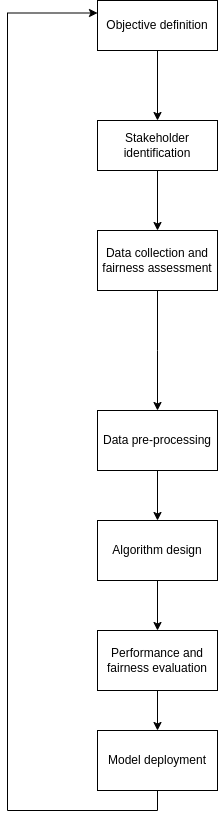
\includegraphics[width=.5\textwidth,height=1\textwidth]{final.png}
    \caption{Fair-by-Design Workflow}
\end{figure}

In the subsequent sections, each of these steps will be comprehensively explored to provide a detailed understanding of the fair-by-design workflow and its ethical underpinnings.

\section{Objective Definition}
\label{section:objective-definition}

The inaugural stage of a fair-by-design workflow mandates the meticulous definition of the system's objectives. The clarity and precision with which these objectives are articulated play a pivotal role in shaping subsequent design decisions. Within the realm of fairness, it becomes imperative to explicitly integrate fairness considerations into the articulated objectives.

In setting the system's goals, a nuanced understanding of the broader ethical landscape becomes foundational. This includes a comprehensive grasp of the potential societal impact, the diverse user base, and the nuanced interplay of ethical considerations within the specific domain of application. The deliberate inclusion of fairness considerations at this early juncture ensures that the pursuit of system objectives aligns seamlessly with the overarching ethical principles, reflecting a commitment to equitable and unbiased outcomes.

By explicitly weaving fairness into the fabric of the defined objectives, the fair-by-design approach underscores its commitment to the proactive anticipation and mitigation of biases. This foundational step lays the groundwork for subsequent design choices, framing the entire development process within an ethical framework that prioritizes fairness and aligns with societal values.

\subsection{Key Considerations}

\begin{enumerate}

    \item \emph{Clarity and Precision:}

        \begin{itemize}

            
            \item \emph{Precision in Objective Definition:} The formulation of specific objectives for the system or process demands clarity and precision to establish a focused and effective approach. This entails articulating goals that are both clear and measurable, aligning seamlessly with the overarching purpose of the system. Objectives should strive to eliminate ambiguity, providing a concrete understanding of the system's intended achievements. 
            
            The significance of clarity in objectives extends beyond the initial definition phase. It serves as a guiding beacon throughout the subsequent development and implementation processes, ensuring a cohesive and purposeful trajectory. Furthermore, the articulation of unambiguous objectives facilitates the accurate evaluation of the system's success in attaining its intended goals. This commitment to precision in objective definition not only enhances the effectiveness of the system but also contributes to a more robust and evaluative framework for assessing its overall impact and success.
            
            \item \emph{Comprehensive Articulation of System Attributes:} A foundational aspect of the fair-by-design workflow involves the explicit and detailed articulation of the system's intended functionalities, goals, and expected outcomes. This comprehensive elucidation is indispensable for fostering a profound understanding of the system or process.

            The delineation of functionalities necessitates a detailed description, outlining the specific tasks or operations the system is designed to execute. Precision in stating goals becomes paramount, emphasizing the overarching aims that the system aspires to achieve. Additionally, the expected outcomes must be clearly defined, specifying the anticipated results or benefits that stakeholders can expect from the successful implementation of the system.
            
            This level of clarity ensures a seamless alignment between development efforts and the envisioned impact, facilitating effective communication and collaboration among all involved parties. By providing a robust framework of understanding, this articulation of functionalities, goals, and outcomes becomes instrumental in guiding subsequent design decisions and ensuring that the fair-by-design approach remains steadfast in its commitment to transparent and equitable system development.        
        
        \end{itemize}
    
    \item \emph{Incorporating Fairness:}

        \begin{itemize}
            
            \item \emph{Explicit Emphasis on Fairness:} A paramount facet in the fair-by-design workflow involves the explicit and emphatic statement of the importance of fairness in achieving the defined objectives. Fairness is not merely an auxiliary consideration; it stands as a foundational principle that underpins the ethical and equitable functioning of the system.

            By explicitly prioritizing fair treatment for all individuals or groups affected by the system, it serves as a cornerstone for enhancing trust, mitigating potential biases, and promoting inclusivity. This acknowledgment of fairness as a non-negotiable element in the pursuit of objectives reflects a resolute commitment to ethical practices and responsible deployment.
            
            Furthermore, positioning fairness as a critical consideration aligns the system with societal values, legal standards, and stakeholder expectations. This alignment not only fosters a positive impact on the system's performance but extends to its broader social implications. The explicit emphasis on fairness within the fair-by-design framework signifies a dedication to cultivating technology that not only meets its functional objectives but does so with a keen awareness of the ethical imperatives that define its relationship with the individuals and communities it serves.
                                    
            \item \emph{Alignment of Fairness with System Purpose:} The seamless alignment of fairness with the overarching purpose of the system is an integral determinant of its effectiveness and societal impact. Fairness ensures that the system operates in a manner characterized by justice, impartiality, and a consideration of diverse perspectives. In this alignment, fairness becomes a cornerstone for enhancing the legitimacy of outcomes, promoting equal opportunities, and guarding against discriminatory practices.

            Incorporating fairness as a core element within the system not only facilitates the ethical attainment of defined objectives but also contributes significantly to cultivating a more inclusive and equitable societal framework. Fairness becomes a driving force that not only strengthens the system's purpose but also fosters trust and positive engagement among users and stakeholders. Simultaneously, it serves as a proactive safeguard, minimizing negative consequences and disparities that may arise from the system's operations.
            
            In essence, the intentional integration of fairness aligns the system with a broader ethical compass, elevating its purpose beyond mere functionality to a realm where societal impact is inherently intertwined with principles of justice, equity, and ethical responsibility.

        \end{itemize}
    
    \item \emph{Balancing Objectives:}

        \begin{itemize}
            
            \item \emph{Balancing Multiple Objectives with Fairness:} Striking a delicate balance among various objectives is paramount, demanding meticulous consideration to prevent the compromise of fairness in the pursuit of other goals. While the system may encompass multifaceted objectives such as efficiency, accuracy, and speed, the commitment to fairness should remain unwavering.

            This delicate equilibrium requires optimizing the system to meet its diverse goals without perpetuating biases or causing harm to specific groups. It necessitates a nuanced approach, where trade-offs are carefully evaluated to ensure that fairness is not sacrificed for the sake of expediency or efficiency. By upholding fairness as a foundational principle, the system can achieve a harmonious equilibrium, fostering an environment where diverse objectives are met without undermining the ethical considerations embedded in the pursuit of those objectives.

            This commitment to balance not only enhances the ethical standing of the system but also contributes to the creation of a technology landscape where fairness is not an afterthought but an integral and non-negotiable aspect of system optimization. In navigating these complexities, the fair-by-design framework becomes a guiding compass, ensuring that the pursuit of efficiency and other objectives remains harmonized with the overarching commitment to fairness.
            
            \item \emph{Identifying Conflicts and Establishing Priorities:} In navigating the intricate landscape of system development, a crucial undertaking involves identifying potential conflicts and establishing priorities among competing objectives. While fairness stands as a paramount consideration, it may at times seem to conflict with other objectives such as efficiency or cost-effectiveness. In such scenarios, conducting a thorough analysis becomes imperative to discern the nature and extent of these conflicts.

            Establishing clear priorities involves a meticulous assessment of the relative importance of each objective and determining where compromises can be made without jeopardizing the ethical principles underpinning fairness. This process demands a careful weighing of trade-offs, with the ultimate goal of aligning competing objectives in a manner that upholds fairness as a non-negotiable priority while still achieving overall system efficiency and effectiveness.
            
            The pursuit of these priorities is not a one-size-fits-all endeavor but requires a nuanced understanding of the specific context and ethical implications. By engaging in this deliberate process of conflict resolution and priority establishment, the fair-by-design workflow ensures that fairness remains at the forefront, serving as a guiding principle that shapes the overall development trajectory of the system.

        \end{itemize}

\end{enumerate}

\subsection{Detailed Implementation Steps}

\subsubsection{Stakeholder Engagement}

\begin{itemize}

    \item \emph{Objective Setting Through Stakeholder Engagement:} The definition of objectives within the fair-by-design workflow is a collaborative and inclusive process that begins by engaging key stakeholders, including end-users, developers, and decision-makers. This fundamental step fosters a collective and participatory approach to system development, where the diverse perspectives and insights of stakeholders are incorporated into the objective-setting process.

    End-users, with their real-world experience, provide valuable input rooted in practical needs. Developers contribute technical expertise, and decision-makers bring strategic considerations to the table. This collective engagement ensures not only a comprehensive understanding of the system's purpose but also enhances the likelihood of creating a solution that aligns with the varied requirements and expectations of all involved parties.

    The collaborative foundation established through stakeholder engagement is essential for achieving consensus on objectives. This consensus, in turn, paves the way for the successful development and implementation of a fair and effective system. By involving stakeholders from the outset, the fair-by-design workflow acknowledges the richness of diverse perspectives, fostering a sense of ownership and collective responsibility in the pursuit of objectives that are both ethically grounded and practically relevant.\item \emph{Objective Setting Through Stakeholder Engagement:} The definition of objectives within the fair-by-design workflow is a collaborative and inclusive process that begins by engaging key stakeholders, including end-users, developers, and decision-makers. This fundamental step fosters a collective and participatory approach to system development, where the diverse perspectives and insights of stakeholders are incorporated into the objective-setting process.

    End-users, with their real-world experience, provide valuable input rooted in practical needs. Developers contribute technical expertise, and decision-makers bring strategic considerations to the table. This collective engagement ensures not only a comprehensive understanding of the system's purpose but also enhances the likelihood of creating a solution that aligns with the varied requirements and expectations of all involved parties.

    The collaborative foundation established through stakeholder engagement is essential for achieving consensus on objectives. This consensus, in turn, paves the way for the successful development and implementation of a fair and effective system. By involving stakeholders from the outset, the fair-by-design workflow acknowledges the richness of diverse perspectives, fostering a sense of ownership and collective responsibility in the pursuit of objectives that are both ethically grounded and practically relevant.
    
    \item \emph{Implementation:}

        \begin{itemize}
            
            \item Conduct stakeholder interviews, surveys, or workshops to gather insights into their expectations and requirements.
            
            \item Ensure diverse representation to capture a comprehensive range of perspectives.
            
            \item Facilitate open discussions to uncover implicit biases or preferences that may influence objectives.
        
        \end{itemize}

\end{itemize}

\subsubsection{Define Performance Metrics}

\begin{itemize}

    \item \emph{Objective:} Specify the metrics that will serve as the yardstick for measuring the success of the system, ensuring a well-defined and quantitative framework for evaluation. These metrics should be meticulously selected to align with the established objectives, encompassing both technical performance and fairness considerations.

    For technical aspects, metrics such as accuracy, precision, recall, and F1 score may be relevant, providing insights into the system's overall effectiveness. Simultaneously, metrics specifically designed to assess fairness, such as disparate impact, equalized odds, and overall fairness indices, should be included to gauge the system's fairness.
    
    The chosen metrics must accurately reflect the intended outcomes and contribute to a comprehensive assessment, enabling a nuanced understanding of the system's success. Upholding fairness as a paramount criterion, the fair-by-design approach ensures that the selected metrics go beyond traditional performance indicators, providing a holistic evaluation that considers both technical proficiency and ethical considerations. This commitment to a diverse set of metrics facilitates a comprehensive understanding of the system's impact, fostering an environment where success is measured not only by technical prowess but also by the ethical principles embedded in the fair-by-design framework.    
    
    \item \emph{Implementation:}
        
    \begin{itemize}
            
        \item Identify traditional performance metrics (e.g., accuracy, precision, recall) relevant to the system's goals.
            
        \item Integrate fairness-specific metrics, such as disparate impact, equalized odds, or statistical parity, depending on the context.
            
        \item Establish a comprehensive set of metrics that collectively address both general system performance and fairness considerations.

    \end{itemize}

\end{itemize}

\subsubsection{Ethical Considerations}

\begin{itemize}

    \item \emph{Objective:} Undertake a comprehensive exploration of the ethical implications associated with the defined objectives, conducting a thorough examination to anticipate and address potential ethical challenges. This involves a deep dive into how the system's goals and functionalities may intersect with broader ethical considerations, including privacy, security, and societal impact.

    Consider the implications for different stakeholder groups, ensuring that the system's objectives align with ethical standards and societal values. This involves a proactive approach, articulating clear guidelines and safeguards to mitigate ethical concerns, thereby promoting transparency and accountability throughout the development and implementation phases.
    
    By proactively addressing ethical implications, the system positions itself to navigate complex ethical landscapes responsibly. This commitment to ethical foresight not only upholds ethical considerations alongside technical functionalities but also contributes to the creation of a technology-driven environment that prioritizes ethical principles. Through this conscientious approach, the fair-by-design workflow not only aims for technical excellence but also seeks to embed a strong ethical foundation, fostering a system that is not only proficient but also ethically responsible.

    \item \emph{Implementation:}

        \begin{itemize}

            \item Conduct an ethical impact assessment to identify potential biases or unintended consequences.

            \item Evaluate the ethical implications of each performance metric, ensuring alignment with fairness goals.

            \item Anticipate scenarios where ethical dilemmas may arise and establish guidelines for resolution.

        \end{itemize}

\end{itemize}

\subsubsection{Documentation}

\begin{itemize}

    \item \emph{Objective:} Rigorously document the defined objectives in a clear and comprehensive manner, ensuring that each objective is articulated with precision and detail. Provide a detailed overview of the intended functionalities, goals, and expected outcomes, leaving no room for ambiguity.

    Utilize concise and unambiguous language to capture the essence of each objective, outlining the specific tasks or functionalities the system aims to achieve. Include any relevant context or background information that enhances the understanding of each objective. This documentation serves as a foundational reference for all stakeholders involved in the development and implementation of the system.

    The goal is to foster a shared understanding of the project's overarching goals and guiding principles among team members, end-users, and decision-makers throughout the system's lifecycle. Clarity and comprehensiveness in objective documentation are indispensable for effective communication and collaboration. By meticulously documenting the objectives, the fair-by-design workflow not only ensures alignment with ethical principles but also establishes a robust foundation for informed decision-making and collective engagement across all stages of system development.
    
    \item \emph{Implementation:}

        \begin{itemize}

            \item Create a detailed objective statement that serves as a reference point for all stakeholders.

            \item Document the rationale behind the inclusion of fairness considerations in the objectives.

            \item Maintain a living document that can be updated as objectives evolve or new insights emerge.

        \end{itemize}

\end{itemize}

\subsection{Significance}

Defining objectives with precision, incorporating fairness considerations, and establishing clear performance metrics are the foundational pillars of a fair-by-design approach. Precision in objective definition is crucial to avoid ambiguity and guide the development process effectively. Integrating fairness considerations from the outset ensures that ethical principles are not an afterthought but integral to the system's purpose. Clear performance metrics enable the systematic evaluation of the system's success and adherence to fairness goals.

Together, these steps create a comprehensive framework that not only aligns the system with ethical standards but also meets stakeholder expectations, fostering trust and accountability throughout the development lifecycle. This approach not only enhances the effectiveness of the system but also contributes to a technology landscape where ethical considerations are seamlessly woven into the fabric of technological advancements. Through a meticulous and proactive fair-by-design methodology, the system becomes not just a product of technical prowess but a testament to ethical responsibility and societal relevance.

\section{Stakeholder Identification}
\label{section:stakeholder-identification}

Engaging key stakeholders is a foundational step in shaping the objectives of a fair-by-design workflow. Stakeholders, representing diverse perspectives and interests, bring invaluable insights that contribute to defining the system's purpose. Involving a range of stakeholders ensures a comprehensive understanding of ethical implications and societal expectations. This inclusive approach not only fosters a sense of collective responsibility but also helps in addressing potential biases and concerns early in the design process.

By incorporating various viewpoints, the fair-by-design workflow becomes more attuned to the needs of different communities and stakeholders, enhancing the overall fairness and effectiveness of the system. This collaborative engagement not only contributes to the ethical grounding of the system but also establishes a sense of shared ownership and accountability among stakeholders. Through this inclusive approach, the fair-by-design methodology ensures that the development process is enriched by a diversity of perspectives, making the resulting system more responsive, transparent, and aligned with the values and expectations of the broader community it serves.

\subsection{Key Considerations}

\begin{enumerate}

    \item \emph{Diverse Representation:}

        \begin{itemize}

            \item \emph{Ensuring Inclusive Stakeholder Representation:} In the fair-by-design approach, ensuring the inclusion of stakeholders who represent a diverse range of perspectives is paramount. This encompasses stakeholders such as end-users, developers, decision-makers, and members of affected communities. Each stakeholder group contributes unique insights and experiences that are crucial for shaping a system that is equitable and aligned with ethical principles.

            End-users provide practical insights into how the system will be experienced, developers offer technical expertise, decision-makers provide strategic guidance, and affected communities bring perspectives on potential societal impacts. By actively involving this diverse set of stakeholders, the fair-by-design workflow gains a more holistic understanding of potential biases, ethical considerations, and the broader societal context, ultimately leading to a more inclusive and equitable outcome.
            
            This intentional inclusion of diverse voices not only enhances the fairness of the system but also establishes a collaborative foundation that reflects a commitment to responsible and ethical AI development. The fair-by-design methodology recognizes the significance of varied perspectives in creating technology that not only functions effectively but also considers the diverse needs and impacts on the communities it serves.

        \end{itemize}
    
    \item \emph{Inclusive Decision-Making:}
        
    \begin{itemize}
    
        \item \emph{Fostering Inclusive Decision-Making:} Fostering an inclusive environment is integral to the fair-by-design approach, ensuring that stakeholders actively participate in decision-making processes related to the system's objectives. This inclusivity encourages diverse perspectives, fostering a collaborative atmosphere where each stakeholder's input is valued.

        Establishing open channels of communication and providing opportunities for meaningful engagement empowers stakeholders to contribute their insights effectively. By creating an inclusive space, the fair-by-design workflow not only captures a broader range of perspectives but also cultivates a sense of ownership among stakeholders. This collaborative decision-making process enhances transparency, builds trust, and ultimately results in a system that is more responsive to the needs and values of the varied stakeholders involved.
        
        Through active and inclusive participation, stakeholders become co-creators of the system, contributing to its development in a manner that reflects a shared commitment to fairness and ethical considerations. This inclusive decision-making not only strengthens the ethical foundation of the system but also fosters a collaborative culture that extends beyond the development phase, influencing the ongoing relationship between the technology and the diverse communities it serves.

    \end{itemize}
    
    \item \emph{Transparent Communication:}
    
    \begin{itemize}

        \item \emph{Maintaining Transparent Communication Channels:} In the fair-by-design approach, maintaining transparent communication channels is crucial to keeping stakeholders informed about the development process and gathering their input effectively. Transparent communication fosters trust and ensures that stakeholders are aware of the system's progress, objectives, and any potential implications.

        Regular updates, clear documentation, and accessible information contribute to an open dialogue, allowing stakeholders to stay engaged and provide valuable feedback. This proactive approach to communication not only enhances the collaborative decision-making process but also promotes a shared understanding of the ethical considerations embedded in the system.
        
        Transparent communication channels serve as a cornerstone of the fair-by-design workflow, fostering a sense of inclusivity and shared responsibility among all stakeholders involved. By keeping the lines of communication open, the fair-by-design methodology not only embraces diverse perspectives but also actively engages stakeholders in a continuous dialogue that extends throughout the system's lifecycle. This commitment to transparency is instrumental in building and sustaining trust, creating an environment where stakeholders feel empowered and informed in their roles as contributors to the ethical development of the technology.

    \end{itemize}

\end{enumerate}

\subsection{Detailed Implementation Steps}

\subsubsection{Stakeholder Mapping}

\begin{itemize}
    
    \item \emph{Objective:} Identifying and mapping key stakeholders is a crucial step in the fair-by-design approach to understand and incorporate diverse perspectives in the system's development. Key stakeholders include end-users, developers, decision-makers, and affected communities, each bringing unique insights and interests to the table.

    End-users provide valuable feedback based on their experiences and expectations, guiding user-centric design. Developers contribute technical expertise, ensuring the feasibility and efficiency of the system. Decision-makers offer strategic input aligning the system with broader organizational goals. Affected communities bring a contextual understanding of societal impacts, helping navigate ethical considerations.
    
    By mapping these stakeholders, the fair-by-design workflow ensures a holistic and inclusive approach, considering the varied interests and perspectives that shape the system's objectives and ethical considerations. This intentional identification and mapping process set the foundation for a collaborative and well-informed decision-making process, where the diverse voices of stakeholders are actively incorporated into the development trajectory of the system.

    \item \emph{Implementation:}
    
    \begin{itemize}
    
        \item Create a stakeholder map that identifies different stakeholder groups and their respective roles and interests.
    
        \item Prioritize stakeholders based on their influence on or impact from the system.
    
    \end{itemize}

\end{itemize}

\subsubsection{Engagement Strategies}

\begin{itemize}

    \item \emph{Objective:} Developing effective strategies for stakeholder engagement in the objective-setting process is pivotal for a fair-by-design workflow. Begin by conducting stakeholder analysis to identify key individuals and groups. Establish clear communication channels to disseminate information and gather feedback. Organize workshops, focus groups, or collaborative sessions to facilitate active participation. Tailor engagement methods to suit diverse stakeholders, ensuring inclusivity.

    Provide accessible documentation outlining the proposed objectives and ethical considerations. Emphasize the value of each stakeholder's input and foster an open dialogue to address concerns. Regularly update stakeholders on the progress, incorporating their feedback iteratively.
    
    By employing these strategies, a fair-by-design workflow ensures comprehensive engagement, enriching the objective-setting process with diverse perspectives and reinforcing ethical considerations. This proactive and inclusive approach to stakeholder engagement not only enhances the quality of the objectives but also contributes to a collaborative and transparent development process, where stakeholders feel valued and actively contribute to the ethical foundation of the system.

    \item \emph{Implementation:}

    \begin{itemize}

        \item Tailor engagement strategies to the characteristics of each stakeholder group (e.g., workshops, surveys, focus groups).

        \item Clearly communicate the importance of their input in shaping the ethical foundations of the system.

    \end{itemize}

\end{itemize}

\subsubsection{Inclusive Workshops or Meetings}

\begin{itemize}

    \item \emph{Objective:} In fostering an inclusive fair-by-design approach, organizing workshops or meetings is instrumental for stakeholder engagement in defining objectives. These sessions provide a platform for active participation, allowing diverse stakeholders, including end-users, developers, decision-makers, and affected communities, to contribute insights.

    The workshops should be designed to encourage open dialogue, ensuring that each perspective is heard and considered. Employ facilitation techniques that promote inclusivity, such as structured discussions, brainstorming sessions, or collaborative activities. By facilitating these inclusive workshops, the fair-by-design workflow embraces diverse viewpoints, enriching the objective-setting process and reinforcing its commitment to ethical considerations.
    
    Through these workshops, the fair-by-design methodology actively encourages a collaborative environment where stakeholders feel empowered to contribute, fostering a sense of ownership and shared responsibility in shaping the system's objectives. This inclusive approach not only enhances the quality of the objectives but also establishes a foundation for continued collaboration and engagement throughout the development lifecycle.

    \item \emph{Implementation:}

    \begin{itemize}

        \item Organize collaborative sessions that encourage open dialogue and the exchange of diverse perspectives.

        \item Provide a platform for stakeholders to express their values, concerns, and expectations related to fairness in the system.

    \end{itemize}

\end{itemize}

\subsubsection{Feedback Collection}

\begin{itemize}

    \item \emph{Objective:} After defining initial objectives and ethical considerations in the fair-by-design workflow, it is crucial to gather feedback from stakeholders. Establish a feedback loop through surveys, interviews, or focus group discussions to ensure that the proposed objectives resonate with the diverse perspectives of stakeholders. This iterative process allows for refinements and adjustments based on the input received.

    Actively seeking feedback fosters collaboration and ensures that the fair-by-design approach remains responsive to the evolving needs and expectations of stakeholders throughout the system's development. This ongoing feedback loop not only contributes to the iterative improvement of objectives but also reinforces a culture of continuous engagement, where stakeholders play an active role in shaping the ethical foundation of the technology.

    \item \emph{Implementation:}

    \begin{itemize}

        \item Utilize surveys, interviews, or online platforms to collect structured feedback.

        \item Encourage stakeholders to provide qualitative insights that may not be captured by quantitative methods.

    \end{itemize}

\end{itemize}

\subsection{Significance}

Stakeholder identification is a pivotal aspect of ensuring the fair and inclusive development of a system. Involving stakeholders from diverse backgrounds and perspectives allows the ethical considerations embedded in the objectives to more accurately reflect the values and expectations of the broader community. By recognizing and engaging with a variety of stakeholders, including end-users, developers, decision-makers, and representatives from affected communities, the fair-by-design approach becomes more comprehensive and responsive to the multifaceted needs and concerns of the people who will interact with or be impacted by the system.

This inclusive process contributes to the development of a system that is not only technically sound but also ethically grounded and considerate of various societal perspectives. The intentional involvement of diverse stakeholders ensures that the resulting technology aligns with ethical standards and is more likely to meet the expectations of the communities it serves, fostering a sense of trust and accountability in the development process.

\section{Data Collection: Integration with Stakeholder Considerations}
\label{section:data-collection}

In the process of data collection, the integration of insights from stakeholders is crucial, particularly for the identification of protected attributes. Stakeholders bring valuable perspectives on societal norms, ethical considerations, and potential biases that may not be apparent solely from the dataset. Their input aids in defining and recognizing protected attributes, contributing to a more nuanced understanding of fairness in the context of the application.

Stakeholder involvement ensures that the identification of protected attributes is not solely based on technical or algorithmic considerations but is informed by the broader societal context. This inclusive approach helps uncover potential biases and ethical implications that might be overlooked in the data, leading to a more robust and ethically grounded system. By actively incorporating stakeholder insights in the identification of protected attributes, the fair-by-design methodology enhances the fairness and accountability of the system, aligning it more closely with the values and expectations of the diverse communities it serves.

\subsection{Importance of Stakeholder Integration}

\subsubsection{Cultural Sensitivity}

Stakeholders, representing diverse backgrounds, contribute significantly to a nuanced understanding of cultural norms and sensitivities within the fair-by-design approach. This diversity is crucial in recognizing attributes that may be culturally significant and warrant protection. For instance, certain cultural or religious practices may involve sensitive information that should be identified as a protected attribute to ensure respectful and unbiased treatment.

By actively involving stakeholders who bring a range of cultural perspectives, the objective-setting process can identify and address potential biases associated with cultural attributes, fostering a system that respects and reflects the rich diversity of its user base. This approach not only enhances fairness but also promotes cultural sensitivity and inclusivity in the design and implementation of the system.

Through the fair-by-design methodology, cultural considerations become integral to the ethical framework, ensuring that the system acknowledges and respects the cultural context of its users. This not only aligns the technology with ethical standards but also contributes to a more inclusive and culturally aware development process, ultimately leading to a system that is more equitable and considerate of the diverse cultural backgrounds of its users.

\subsubsection{Contextual Relevance}

Stakeholders play a crucial role in providing contextual insights that may not be evident in the dataset alone within the fair-by-design approach. Their considerations can guide the identification of attributes relevant to the specific application and its ethical implications. For instance, in an educational context, stakeholders might highlight attributes related to socio-economic status or learning styles that could impact fairness considerations in student evaluations.

By actively involving stakeholders, the objective-setting process gains valuable perspectives that enrich the ethical framework of the system. This collaborative approach ensures that the identified objectives not only align with technical requirements but also address real-world considerations, promoting a more holistic and socially responsible system.

Through the fair-by-design methodology, stakeholders become partners in shaping a system that is not only technically robust but also considerate of the diverse and dynamic factors influencing its ethical considerations. This inclusive collaboration helps bridge the gap between technical requirements and real-world implications, fostering a technology landscape that is not only advanced but also socially conscious and responsive to the needs and concerns of the communities it serves.

\subsubsection{Uncovering Implicit Biases}


Stakeholders play a crucial role in uncovering implicit biases that may not be explicitly represented in the dataset within the fair-by-design approach. By incorporating their perspectives, the identification of protected attributes becomes more comprehensive and reflective of potential sources of bias. This is particularly important in domains where historical biases or societal prejudices might influence decision-making processes.

Stakeholders can provide valuable input to address and mitigate these implicit biases, contributing to the development of a more equitable and unbiased system. Their involvement ensures a thorough examination of potential biases, fostering transparency and fairness in the system's design and objectives.

Through the fair-by-design methodology, stakeholders act as critical agents in the identification and mitigation of biases, leading to a more robust and ethically grounded system. This collaborative approach not only enhances the fairness of the technology but also promotes a culture of accountability and transparency in addressing biases that may exist in the underlying data or decision-making processes.

\subsection{Implementation Steps}

\subsubsection{Stakeholder Workshops}

\emph{Objective:} Integrate stakeholder considerations into the identification of protected attributes.

\emph{Implementation:}

\begin{itemize}

    \item Conduct stakeholder workshops specifically focused on discussing and identifying potential protected attributes.

    \item Encourage open discussions to uncover implicit biases or attributes that may have societal implications.

    \item Facilitate collaboration between data scientists and stakeholders to ensure a shared understanding of fairness goals.

\end{itemize}

\subsubsection{Documentation of Stakeholder Input}

\emph{Objective:} Document stakeholder input on protected attributes for transparency.

\emph{Implementation:}

\begin{itemize}

    \item Record the insights shared by stakeholders regarding attributes they perceive as sensitive or requiring protection.

    \item Incorporate stakeholder considerations into the broader documentation of the data collection process.

    \item Provide clear documentation of the integration process to maintain transparency and facilitate reproducibility.

\end{itemize}

\section{Data Pre-processing}
\label{section:pre-proc}

Following the completion of data collection and the incorporation of stakeholder considerations, the subsequent pivotal stage in the workflow is data pre-processing. This critical phase is dedicated to meticulously preparing and cleansing the dataset with the overarching goal of addressing biases, rectifying imbalances, and ensuring a fair and equitable foundation for the ensuing stages of the fair-by-design workflow. The emphasis during data pre-processing is on refining the dataset to foster a more equitable and unbiased representation, thus laying the groundwork for robust and ethical data-driven decision-making processes.

\subsection{Key Considerations}

\begin{enumerate}

    \item \emph{Data cleaning:} 

    This process involves identifying and rectifying errors, inconsistencies, and inaccuracies in the raw dataset to ensure its reliability and quality. Common tasks in data cleaning include handling missing values, correcting data format issues, removing duplicates, and addressing outliers. The goal is to create a clean, standardized dataset that forms a solid foundation for subsequent analysis and model development. Rigorous data cleaning is essential for mitigating the risk of biased or inaccurate model outcomes, as machine learning models heavily depend on the quality of the input data. This meticulous attention to data quality sets the stage for effective feature engineering, model training, and, ultimately, the generation of reliable and fair predictions.

    \item \emph{Handling Protected Attributes:} 
    
    Within the Fair-by-Design workflow, categorical protected attributes undergo a transformation process to ensure fairness in subsequent machine learning stages. This process involves setting a threshold for each protected attribute and replacing values above the threshold with 1, and values below the threshold with 0.

    Let \(P\) be the set of protected attributes, and \(p_i\) represent a specific protected attribute within \(P\). The threshold, denoted as \(t_i\), is determined for each categorical protected attribute \(p_i\) in the dataset through the following formalism:

    \[

    t_i = \frac{\text{min}(p_i) + \text{max}(p_i)}{2}
    
    \]

    This calculation ensures a nuanced understanding of the prevalent categories within these attributes and establishes a threshold \(t_i\) for distinguishing between them.

    The binary representation preserves essential information about protected attributes, providing a condensed yet informative encoding that reflects the privilege or lack thereof concerning specific attributes.

    During the training phase, the model learns to distinguish instances based on privilege or lack thereof concerning specific attributes, as represented by the binary encoding. This is achieved by replacing values according to the following transformation:

    \[

    \text{Binary Encoding}(p_i) = \begin{cases} 

        1 & \text{if } p_i \geq t_i \\

        0 & \text{if } p_i < t_i 

    \end{cases}

    \]

    This facilitates effective model incorporation and decision-making during training and prediction phases.

    The nuanced encoding strategy, where values over the threshold are replaced with 1 and values under the threshold are replaced with 0, serves as the foundation for unbiased and fair treatment of instances within the model. By transforming categorical protected attributes based on the specified threshold definition, the Fair-by-Design workflow ensures that subsequent machine learning models can effectively incorporate and act upon this information during training and prediction phases, contributing significantly to the development of a more equitable and ethically sound machine learning model.

    \item \emph{Handling Output Variable:} 
    
    The handling of the output variable in the Fair-by-Design workflow is a nuanced process that adapts to the nature of the variable, whether categorical or continuous. This tailored treatment is essential for aligning the prediction task with the fairness objectives of the workflow, ensuring that the model's predictions are not only accurate but also ethically sound.


    In cases where the output variable is categorical, the workflow initiates by determining the most frequent value within this category. Let $Y$ represent the output variable, and $y_i$ be a specific outcome within $Y$. The most frequent value, denoted as $y_{\text{freq}}$, is determined through the following formalism:

    \[
    y_{\text{freq}} = \text{argmax}_y \left( \text{count}(Y = y) \right)
    \]

    This strategic calculation provides insights into the prevailing outcome within the dataset. Subsequently, instances where the output variable matches $y_{\text{freq}}$ are replaced with the binary representation 1, while all other instances take on the binary representation 0. The binary encoding function is defined as follows:

    \[
    \text{Binary Encoding}(y_i) = \begin{cases} 
    1 & \text{if } y_i = y_{\text{freq}} \\ 
    0 & \text{otherwise}
    \end{cases}
    \]

    This transformation effectively redefines the prediction task, shifting the focus to discerning whether a given sample belongs to the most frequent outcome. The binary encoding approach not only simplifies the representation of categorical outcomes but also enables the model to make predictions in a manner that aligns with fairness considerations.


    Conversely, when the output variable is continuous, the workflow employs a distinct strategy. Let $Z$ represent the continuous output variable, and $z_i$ be a specific value within $Z$. Values of the continuous variable that surpass the mean are replaced with 1, while those falling below the mean assume the binary representation 0. This adjustment transforms the prediction task into establishing whether a sample's continuous output is above the mean. The binary encoding function for continuous variables is defined as:

    \[
    \text{Binary Encoding}(z_i) = \begin{cases} 
    1 & \text{if } z_i > \text{mean}(Z) \\ 
    0 & \text{otherwise}
    \end{cases}
    \]

    This approach ensures that the model is not only attentive to the central tendency of the continuous variable but also considers the distribution of values concerning the mean.

    This tailored and meticulous treatment of the output variable underscores the commitment of the Fair-by-Design workflow to equitable and ethical machine learning practices. The workflow not only adapts to the inherent characteristics of the data but also ensures that the subsequent model operates with a heightened awareness of fairness considerations, contributing to the development of a more responsible and unbiased machine learning model.

\end{enumerate}

This nuanced pre-processing step sets the groundwork for a fair and unbiased learning prediction, aligning the dataset with the ethical considerations embedded in the Fair-by-Design workflow.

\section{Algorithm Design}
\label{section: algorithm-design}

The stage of Algorithm Design within the fair-by-design workflow stands as a pivotal phase wherein the selection, adaptation, or creation of machine learning models takes place to harmonize with the specified objectives and fairness considerations. The primary objective is to craft models that not only excel in accuracy but also steadfastly adhere to ethical and fair principles. This section undertakes an in-depth exploration of the crucial considerations, strategic approaches, and the step-by-step implementation processes entailed in Algorithm Design. By navigating through these aspects, the aim is to foster the development of models that not only deliver superior performance but also champion the ideals of ethics and fairness in their predictive outcomes.

\subsection{Key Considerations}

\begin{enumerate}

    \item \emph{Fairness-Aware Model Selection:} 
    
    The selection of machine learning models assumes a pivotal role in the pursuit of fairness objectives. Fairness-aware model selection entails the deliberate consideration of models equipped with inherent mechanisms to tackle biases and advocate for equitable outcomes. Noteworthy examples of such models include adversarial networks, fairness-aware classifiers, and re-weighted learning algorithms. These models are systematically explored and evaluated for their capacity to mitigate biases and foster fairness, thereby contributing to the overarching goal of cultivating just and impartial predictive systems.
    
    \item \emph{Regularization Techniques:} 
    
    In the pursuit of fair predictions, regularization methods, exemplified by demographic parity constraints or equalized odds constraints, emerge as instrumental tools. These methodologies are strategically employed to guide machine learning models towards fairness objectives. By integrating fairness constraints into the optimization process, these regularization techniques play a pivotal role in steering the model to yield equitable outcomes across various demographic groups. The inclusion of such constraints serves as a proactive measure to counteract biases and ensure that the predictive power of the model remains impartial and just across diverse demographic contexts.

    \item \emph{Bias Detection and Mitigation:} 
    
    The integration of embedding mechanisms within the algorithm to detect and mitigate biases is of paramount importance. This entails the ongoing and systematic monitoring of the model's predictions for any indications of disparate impact. Subsequently, corrective measures are implemented in real-time to mitigate biases as they manifest. This proactive approach to bias detection and mitigation serves as a fundamental component in ensuring the model's fairness and equity. By embedding mechanisms that facilitate continuous scrutiny and timely interventions, the algorithm is fortified to deliver more impartial and just predictions, aligning with the principles of ethical and fair machine learning.

    \item \emph{Pre-processing, In-processing, or Post-processing Algorithms:} 
    
    The strategic decision regarding the selection of pre-processing, in-processing, or post-processing algorithms is intricately tied to the specific characteristics of the data and the defined fairness goals. Pre-processing algorithms, characterized by their ability to transform the dataset prior to model training, set the initial conditions for fairness considerations. In-processing algorithms, on the other hand, directly modify the learning process during model training, introducing fairness mechanisms at this crucial stage. Post-processing algorithms, as the name implies, come into play after model training, adjusting predictions to align with fairness objectives.

    When making this strategic decision, it is imperative to consider the nature of biases inherent in the data, the characteristics of the available dataset, and the desired level of fairness. Each approach—pre-processing, in-processing, or post-processing—offers distinct advantages and considerations, and the choice among them should be informed by a comprehensive understanding of the specific fairness challenges and objectives inherent to the machine learning task at hand.

\end{enumerate}

\subsection{Detailed Implementation Steps}

% Include the detailed implementation steps for each key consideration as per the previous discussion.

\subsubsection{Fairness-Aware Model Selection}

\begin{itemize}

    \item \emph{Exploration of Fairness-Aware Models:}
     
    \begin{itemize}
    
        \item In the endeavor to develop a fair-by-design machine learning model, a pivotal step involves conducting an exhaustive survey and evaluation of existing fairness-aware models tailored to the specific application domain. This meticulous process requires a thorough examination of pertinent literature and available models, taking into account their performance metrics, interpretability, and fairness considerations. By subjecting existing models to rigorous evaluation, practitioners gain valuable insights into the nuanced strengths and limitations of different approaches. This discerning survey and evaluation process empower practitioners to make informed decisions regarding the most suitable model for their particular use case. Such diligence contributes significantly to the foundational aspects of a fair-by-design workflow, ensuring that the selected model not only aligns with technical requirements but also upholds ethical considerations inherent to the application domain.
    
        \item When delving into the realm of fairness-aware models tailored for a specific application domain, it is judicious to prioritize models explicitly designed to address bias. This consideration encompasses, but is not confined to, adversarial networks or models featuring inherent fairness constraints. Adversarial networks serve the purpose of mitigating bias by introducing a secondary network that identifies and counteracts any discriminatory patterns discerned in the primary model. Conversely, models with built-in fairness constraints integrate predefined fairness metrics into the optimization process, ensuring the model adheres to fairness criteria throughout training.

        The evaluation of these specialized models yields a nuanced understanding of their efficacy in handling bias, furnishing practitioners with invaluable insights into the most suitable approach for mitigating bias within their specific context. This deliberate consideration solidifies the fair-by-design approach, underscoring the paramount importance of selecting models that actively address and rectify biases to foster equitable outcomes in the realm of machine learning applications.    
    
    \end{itemize}
    
    \item \emph{Implementation and Customization:}
    
    \begin{itemize}
    
        \item Following the selection of a fairness-aware model tailored for the specific application domain, the subsequent imperative involves its implementation within the chosen machine learning framework. This intricate process necessitates the translation of model specifications and architecture into code, meticulous configuration of essential parameters, and seamless integration into the overarching machine learning pipeline. The implementation procedure should strictly adhere to industry best practices and guidelines stipulated by the chosen framework, ensuring not only optimal performance but also seamless compatibility.

        Furthermore, developers must prioritize the interpretability of the model, recognizing that transparency is pivotal in comprehending how fairness considerations are intricately embedded within the system. The successful execution of the implementation phase represents a pivotal juncture in the fair-by-design workflow. It sets the groundwork for subsequent stages encompassing model training, rigorous evaluation, and eventual deployment, all underscored by an unwavering commitment to fostering equitable and unbiased machine learning outcomes.    
    
        \item Subsequent to the implementation of the chosen fairness-aware model, a pivotal phase entails customizing the model to harmonize with the unique characteristics of the dataset and the precise fairness objectives delineated earlier in the workflow. This customization process necessitates the fine-tuning of model parameters, adjustment of hyperparameters, and incorporation of features that aptly accommodate the nuanced intricacies present in the dataset.

        Moreover, developers may find it imperative to introduce specific fairness-oriented adjustments to the model's architecture. This ensures the model's adeptness in effectively handling and mitigating biases associated with protected attributes. Such meticulous and tailored customization stands as an indispensable step for optimizing the model's performance within the paradigm of the fair-by-design approach. Here, the overarching objective extends beyond technical excellence, encompassing the ethical imperative of delivering unbiased machine learning outcomes.    
    
    \end{itemize}

\end{itemize}

\subsubsection{Explainability and Interpretability}

\begin{itemize}

    \item \emph{Model Selection:}

    \begin{itemize}

        \item Within the fair-by-design workflow, the strategic choice of models renowned for their high explainability and interpretability holds paramount significance. Decision trees and rule-based models, celebrated for their inherent transparency, stand out as preferred choices in this context. The rationale underpinning this selection is deeply rooted in the commitment to transparency and accountability.

        Models characterized by easy interpretability empower stakeholders, including end-users and decision-makers, to comprehend the intricate decision-making processes. This transparency not only cultivates trust but also facilitates the identification and mitigation of any potential biases or fairness concerns embedded within the model. By deliberately opting for models with high explainability, the fair-by-design workflow aligns seamlessly with its overarching goal of cultivating machine learning systems that excel not only in technical robustness but also in ethical soundness, ensuring they are readily understandable by a diverse range of stakeholders.

        \item Within the fair-by-design workflow, when infusing fairness considerations into model selection, a critical aspect is to judiciously navigate the trade-offs between model complexity and interpretability. The optimal balance hinges significantly on the specific application requirements, playing a pivotal role in the decision-making process.

        Highly complex models, while potentially offering superior predictive performance, often come at the cost of diminished interpretability. Conversely, interpretable models such as decision trees or rule-based models may exhibit limitations in capturing intricate patterns present in the data. Striking the right balance becomes paramount; the fair-by-design approach is not solely concerned with ensuring fairness but also places a premium on transparency.
        
        Therefore, the strategic selection of models aligning with the interpretability needs of stakeholders while still meeting performance requirements becomes a key consideration in the design process. This deliberate and conscious decision-making process contributes significantly to the development of machine learning models that are not only fair but also understandable and accountable, embodying the principles of the fair-by-design approach.

    \end{itemize}

\end{itemize}

\subsubsection{Regularization Techniques}

\begin{itemize}

    \item \emph{Integration of Fairness Constraints:}

    \begin{itemize}

        \item The incorporation of fairness constraints mandates a nuanced comprehension of the precise fairness goals and metrics germane to the application domain. In the fair-by-design approach, there is a pronounced emphasis on the principled and systematic integration of these constraints into the machine learning model's training process. This deliberate embedding of fairness into the training regimen aims to mitigate biases and advocate for equitable outcomes.

        The overarching objective of the fair-by-design workflow extends beyond the mere delivery of accurate predictions. It is intricately woven with the commitment to ethical and fairness considerations, thereby contributing substantively to the cultivation of responsible and unbiased machine learning practices. This concerted effort reinforces the imperative of aligning machine learning models with ethical principles, ensuring they operate within a framework that prioritizes fairness and equity.

        \item Within the fair-by-design approach to machine learning, a pivotal facet involves the systematic experimentation with various regularization techniques. These methods, exemplified by demographic parity constraints or equalized odds constraints, assume a substantial role in the concerted effort to mitigate biases and champion fairness within machine learning models. Tailored to address specific fairness considerations linked to protected attributes, these techniques are meticulously designed to ascertain that the model's predictions remain uninfluenced by factors such as gender, race, or other sensitive attributes. This intentional and exploratory engagement with regularization techniques underscores the commitment to cultivating models that not only excel in predictive accuracy but also uphold the ethical imperative of fairness and equity.
    
    \end{itemize}

\end{itemize}

\subsubsection{Bias Detection and Mitigation}

\begin{itemize}
    
    \item \emph{Dynamic Bias Mitigation:}
    
    \begin{itemize}
    
        \item A proactive strategy within the fair-by-design framework involves the development of adaptive algorithms that dynamically adjust to emerging biases in the data. These algorithms are meticulously designed to engage in continuous monitoring and evaluation of the model's performance, adept at identifying any potential biases that may manifest during operational phases. The adaptive nature of these algorithms empowers them to dynamically tweak parameters or decision boundaries in response to emerging biases, thereby ensuring an ongoing commitment to fairness in real-world applications. This forward-thinking approach aligns seamlessly with the ethos of the fair-by-design framework, emphasizing not only initial fairness but also the continuous vigilance and adaptation necessary for sustained equity in machine learning outcomes.

        \item A pivotal step in the fair-by-design workflow involves the implementation of corrective measures, such as re-weighting or re-sampling, to actively mitigate biases as they are detected. As biases are identified through ongoing monitoring, these targeted corrective measures are strategically applied to address imbalances and promote fairness in the model's predictions. This iterative and adaptive approach not only acknowledges the inevitability of biases but also proactively works towards rectifying them, reinforcing the commitment to fairness and equity embedded within the fair-by-design methodology.

    \end{itemize}

\end{itemize}

\subsubsection{Human-in-the-Loop Approaches}

\begin{itemize}
    
    \item \emph{Stakeholder Collaboration:}
    
    \begin{itemize}
    
        \item Organize collaborative sessions with domain experts and stakeholders to delve into the intricacies of fairness considerations. These sessions serve as a platform for a comprehensive exploration of nuances related to fairness, leveraging the collective insights and expertise of domain specialists and key stakeholders. The aim is to foster a shared understanding of fairness challenges, identify contextual nuances, and coalesce diverse perspectives. Such collaborative endeavors contribute significantly to the fair-by-design approach, ensuring that the developed models align not only with technical requirements but also with the ethical and contextual considerations of the specific application domain.
    
        
        \item Engage stakeholders actively in both model validation and decision-making processes. This participatory approach ensures that the perspectives and insights of stakeholders are integral to the validation of the model's performance and the decision-making procedures. By involving stakeholders, including end-users and decision-makers, in these crucial stages, the fair-by-design workflow embraces transparency and inclusivity. This collaborative involvement contributes to the development of models that are not only technically sound but also align with the diverse needs and expectations of the stakeholders, fostering a sense of ownership and accountability in the overall machine learning process.
    
    \end{itemize}

\end{itemize}

\subsection{Pre-processing Algorithm Proposed}

\subsubsection{Fairness through data rebalancing}
\label{subsec:ftdr}

In this approach, the paradigm of bias mitigation takes on a unique and innovative perspective, one that prioritizes data augmentation over attribute removal. Unlike traditional approaches that center on the exclusion of specific attributes, this methodology embraces the concept of data augmentation, introducing a distinctive definition of fairness and equity within the AI system.

The essence of this approach revolves around the augmentation of the dataset by introducing new data instances that offer a more comprehensive and inclusive representation of the underlying population. This expanded dataset is designed to be more diverse, representative, and balanced, transcending the limitations of the original data and fostering a more nuanced understanding of fairness. 

The introduction of augmented data instances leads to a redefined notion of fairness within the AI system. Instead of solely focusing on the absence of biased attributes, fairness is now measured in terms of the dataset's inclusivity and its ability to capture the diversity and nuances present within the population it seeks to serve. 

This approach aligns with the broader philosophy of ensuring that AI systems are equitable, just, and capable of making informed and unbiased decisions. By augmenting the dataset, it strives to bridge the gaps in representation and provide a more equitable playing field for all individuals, regardless of their background or characteristics. 

The process of data augmentation necessitates a careful selection of techniques and methodologies that can introduce new data instances while maintaining the integrity and quality of the dataset. These techniques may encompass oversampling, synthetic data generation, or other data synthesis methods, each tailored to the specific context and objectives of the AI system.

In traditional fairness definitions, the focus often revolves around ensuring fair treatment for individual protected attributes, denoted as $A_1, A_2, \ldots, A_k$. While this is undoubtedly crucial, a more comprehensive understanding of fairness calls for an examination of fairness in the context of combinations of protected attributes and the output. A new definition of fairness is proposed, which takes into account the representation of all combinations of $k$ protected attributes and the output, aiming for equitable representation across these combinations.

A fair dataset is defined as one in which, for each combination of protected attributes $\{A_1, A_2, \ldots, A_k\}$ and the output $O_j$, the representation is equal and proportional. Mathematically, a dataset is fair if:

\[
\forall i_1, i_2, \ldots, i_k, j: \frac{|D_{i_1, i_2, \ldots, i_k, j}|}{|D|} = \text{constant}
\]

where:
- $D$ is the dataset,
- $|D_{i_1, i_2, \ldots, i_k, j}|$ is the number of samples with the specific combination of protected attributes $A_{i_1}, A_{i_2}, \ldots, A_{i_k}$ and output $O_j$,
- $|D|$ is the total number of samples in the dataset.

This entails that any combination of demographic groups, defined by the protected attributes, and the output should have comparable representation, thereby fostering a balanced and unbiased dataset.

By striving for equal representation of combinations of protected attributes, is addressed a fundamental aspect of fairness that transcends individual attributes. This approach provides a more nuanced understanding of fairness by considering the intersections of various demographic groups. It encourages a broader examination of potential biases that may arise when considering multiple attributes simultaneously.

Incorporating this definition of fairness into the dataset rebalancing process enables us to promote a comprehensive notion of fairness, aligning with the principles of equal opportunity and non-discrimination across all combinations of protected attributes. The subsequent algorithm and experimental evaluation are designed to actualize this definition and demonstrate its effectiveness in achieving a more equitable representation within the dataset.

At this point it's necessary to begin with a formalization for the algorithm itself.


Let \( D \) be a dataset \( R^{n \times m} \), where \( n \) is the number of samples and \( m \) is the number of features. Let \( k \) be the number of protected variables represented as \( R^{n \times 1} \), and let there be a single output variable represented as \( R^{n \times 1} \).

A rebalancing function \( \mathcal{R} \) can be formally defined as a mapping:

\[
\mathcal{R}: R^{n \times m} \rightarrow R^{l \times m}
\]

where \( l > m \), and the function \( \mathcal{R} \) transforms the input dataset \( D \) of dimensions \( n \times m \) into an output dataset \( D' \) of dimensions \( l \times m \).



Let \( k \) be the number of binary protected variables in the dataset \( D \), and consider the output variable to be binary as well. The number of possible combinations of these variables is \( 2^{(k+1)} \).

Consider a set \( \text{Combination-frequency} \) with occurrences of all \( 2^{(k+1)} \) combinations within the dataset. For each combination, the number of rows in which that combination appears should be equal to the maximum occurrence among all combinations present in the set \( \text{Combination\textunderscore frequency} \). This maximum value is denoted as \( \text{Max}(\text{Combination-frequency}) \).

Mathematically, the number of rows (\( l \)) the final dataset should have for each combination is given by:

\[
l = \text{Max}(\text{Combination-frequency})
\]



Let \( l \) be the desired number of rows for the final dataset. For each combination of values, is calculated the occurrence count \( \text{occurrence}_i \), where \( i \) ranges from 1 to \( 2^{(k+1)} \), with \( k \) being the number of protected binary variables and considering the output variable as binary.

The total number of rows to be added is given by:

\[
\text{total\_rows\_to\_add} = l - \sum_{i=1}^{2^{(k+1)}} \text{occurrence}_i
\]

For each iteration:

\begin{itemize}

    \item The values of the protected and output variables are set according to the specific combination.
    
    \item For all other attributes, a random value \( \text{random\_value}_{ij} \) is generated, where \( j \) represents the specific attribute and \( i \) represents the row being added for that attribute. \( \text{random\_value}_{ij} \) is within the minimum and maximum range for attribute \( j \).

\end{itemize}

As showed in the following pseudocode

\begin{algorithm}[H]
    \caption{Reabalancing}
    \begin{algorithmic}[1]
        \State \textbf{Input:} combination\_set, combination\_frequency, protected\_attributes, dataset\_attributes
        \State \textbf{Output:} Updated dataset

        \State max\_frequency $\gets$ max(combination\_frequency)

        \For{index \textbf{in} (0, len(combination\_set) - 1)}
            \State combination $\gets$ combination\_set[index]
            \State frequency $\gets$ combination\_frequency[index]
            \State combination\_dataset $\gets$ dataset[dataset[combination] == combination\_set[index]]

            \While{frequency $<$ max\_frequency}
                \State new\_row $\gets$ empty

                \For{(attr, val) \textbf{in} (combination, protected\_attributes)}
                    \State new\_row[attr] $\gets$ val
                \EndFor

                \For{attr \textbf{in} dataset\_attributes \textbf{and not in} protected\_attributes}
                    \State new\_row[attr] $\gets$ random(min(combination\_dataset[attr]), max(combination\_dataset[attr]))
                \EndFor

                \State dataset.add(new\_row)
                \State frequency $+$= 1
            \EndWhile
        \EndFor

        \State \textbf{return} Updated dataset
    \end{algorithmic}
\end{algorithm}

this algorithm adds rows to the dataset until every combination have the same frequency. Fundamental for this algorithm is the way in which are generate the value for the variables not involved into the combination. These are added considering the sub-dataset of the original dataset in which the combination occurs. 


\subsection{Significance}

The Algorithm Design stage is pivotal in shaping the ethical and fair behavior of machine learning models within the fair-by-design framework. By carefully selecting, customizing, and integrating fairness-aware models, and incorporating transparency and human-in-the-loop approaches, this stage ensures that the resulting models align with ethical considerations and promote equitable outcomes.

\section{Model Training and Evaluation}
\label{section:model-training}

\subsection{Introduction}

This section delivers a thorough overview of the model training and evaluation process within the Fair-by-Design framework. After the careful application of the chosen pre-processing, in-processing, or post-processing algorithm, the training phase assumes a pivotal role in shaping a machine learning model. The emphasis extends beyond mere accuracy objectives to incorporate the ethical considerations of fairness. This holistic approach underscores the commitment to developing models that excel not only in predictive performance but also adhere to principles of equity and justice, thereby embodying the ethos of the Fair-by-Design framework.

\subsection{Training Process}

\subsubsection{Data Splitting}

The dataset undergoes a deliberate split into training, validation, and test sets, each serving a distinct strategic purpose. The training set acts as the foundation for the model's learning process, enabling it to grasp patterns and relationships within the data. The validation set plays a crucial role in hyperparameter tuning, fine-tuning the model to enhance its generalization capabilities. Finally, the test set serves as the litmus test for the final model's performance, offering a reliable measure of its predictive capabilities. This meticulous division ensures a comprehensive and robust evaluation of the model's effectiveness and generalizability within the Fair-by-Design framework.

\subsubsection{Model Architecture}

The architecture of the selected model is meticulously crafted to strike a delicate balance between accuracy and fairness considerations within the Fair-by-Design framework. Architectures may incorporate innovative components, such as adversarial layers or customized modules specifically designed to enforce fairness constraints. The focal point is to develop a model that excels not only in capturing intricate patterns but is also interpretable and transparent in its decision-making process. This intentional design reflects the commitment to fostering models that go beyond predictive prowess, embodying principles of interpretability and transparency while addressing fairness concerns.

\subsubsection{Training Parameters}

Critical training parameters, spanning the learning rate, batch size, and convergence criteria, undergo meticulous tuning in the Fair-by-Design framework. The learning rate assumes significance as it dictates the step size in the optimization process, thereby influencing the pace of updates to model parameters. This parameter is pivotal in determining the balance between the model's adaptability and stability during training.

The batch size, another key parameter, determines the number of samples processed in each iteration. This factor significantly impacts the overall efficiency of the training process, influencing resource utilization and the model's ability to generalize well to diverse datasets.

Convergence criteria hold a crucial role by ensuring that the training process halts when the model achieves optimal performance. These criteria are indispensable in preventing overfitting, safeguarding against the model becoming excessively tailored to the training data to the detriment of its ability to generalize to new, unseen data.

This comprehensive tuning process, applicable beyond deep models, reflects a nuanced approach in optimizing key parameters to foster models that not only exhibit accuracy but also align with fairness considerations in the Fair-by-Design paradigm.

\subsubsection{Fairness Constraints}

In scenarios where fairness constraints are seamlessly integrated into the training process within the Fair-by-Design framework, a deliberate and systematic approach is adopted. These constraints are explicitly defined and enforced, often involving the introduction of regularization terms designed to penalize disparate treatment of different demographic groups. This strategic incorporation aims to instill fairness by discouraging the model from exhibiting biased behavior towards specific groups.

Adversarial training components might also be leveraged in this process. These components act as a countermeasure to mitigate bias, introducing a dynamic element that works to identify and neutralize any discriminatory patterns that may emerge during training. The overall objective is to foster models that not only deliver accurate predictions but also adhere to ethical principles of fairness and equity. This intentional integration of fairness constraints reinforces the commitment to cultivating machine learning models that contribute to just and unbiased outcomes.

\subsubsection{Model Training}

The model undergoes training for a specified number of iterations, leveraging the training set to iteratively update its parameters and increase accuracy. This iterative training process is not limited to deep learning models and is applicable across various model categories. The overarching goal remains to strike a balance between accuracy and fairness, contributing to the development of a machine learning model proficient in capturing underlying patterns while being conscious of potential biases.

Through successive iterations on the training set, the model refines its understanding of the data, aiming to optimize its performance with due consideration to fairness. This approach aligns with the principles of the Fair-by-Design framework, ensuring that the trained model is both technically robust and ethically sound in its decision-making, irrespective of the specific model category employed.

\subsection{Evaluation Metrics}

\subsubsection{Accuracy Metrics}

A suite of accuracy metrics is employed to holistically assess the model's overall performance:

\begin{itemize}
    \item \emph{Accuracy:} The ratio of correctly predicted instances to the total instances.
    
    \item \emph{Precision:} The proportion of true positive predictions among instances predicted as positive.
    
    \item \emph{Recall:} The proportion of true positive predictions among actual positive instances.
    
    \item \emph{F1-score:} The harmonic mean of precision and recall, providing a balanced measure of accuracy.
\end{itemize}

\subsubsection{Fairness Metrics}

Fairness metrics are instrumental in evaluating the model's behavior across different demographic groups:

\begin{itemize}
    
    \item \emph{Equalized Odds Evaluation Metric}: The Equalized Odds metric serves as a critical assessment tool for gauging the model's performance concerning fairness. This evaluation metric specifically investigates whether the model exhibits comparable false positive and false negative rates across distinct demographic groups. By scrutinizing disparities in these rates, the Equalized Odds metric offers insights into the model's capacity to provide equitable outcomes for diverse segments of the population, contributing to a comprehensive understanding of its fairness considerations, as reported in \cref{section:metrics}
    
    \item \emph{Statistical Parity:} The Statistical Parity metric is a meticulous examination of the distribution of positive outcomes within each demographic group. This evaluation metric meticulously analyzes the proportion of positive results for each group, aiming to identify and quantify any disparities that may exist. By shedding light on these disparities, the Statistical Parity metric offers a nuanced perspective on how the model's predictions align with different demographic segments. This in-depth analysis contributes to a comprehensive assessment of fairness, facilitating a more detailed understanding of potential imbalances in positive outcomes across diverse groups, as reported in \cref{section:metrics}

\end{itemize}

\subsection{Results and Analysis}

\subsubsection{Accuracy Results}

A meticulous analysis of accuracy results stands as a cornerstone in gaining valuable insights into the model's predictive prowess concerning the target variable. Precision, recall, and F1-score metrics play a pivotal role in offering a nuanced understanding of the intricate trade-offs between true positives, false positives, and false negatives.

Precision provides insights into the accuracy of positive predictions, recall assesses the model's ability to capture all positive instances, and the F1-score encapsulates a harmonized view, considering both precision and recall. The overarching goal transcends mere accuracy; it extends to cultivating a balanced and informed prediction capability. This multifaceted evaluation approach ensures a comprehensive grasp of the model's performance, allowing for a nuanced interpretation of its predictive accuracy while considering the intricate interplay between different performance metrics.

\subsubsection{Fairness Results}

Fairness metrics serve as a crucial lens through which biases within the model are identified and addressed. Disparate impact, equalized odds, and statistical parity results undergo thorough analysis to evaluate whether the model demonstrates disparate treatment among various demographic groups. The emphasis is not only on recognizing but also on actively mitigating disparities, fostering the development of a model that upholds principles of fairness and equity. By leveraging these metrics, the evaluation process goes beyond traditional performance measures, ensuring a diligent scrutiny of how the model's predictions may impact different demographic segments and actively working towards an unbiased and equitable predictive system.

\subsubsection{Trade-offs}

Comprehending the nuanced trade-offs between accuracy and fairness is pivotal in the pursuit of a balanced model. Achieving this equilibrium may necessitate adjustments to the model. Techniques such as re-weighting, re-sampling, or the introduction of customized loss functions can be employed to specifically address fairness concerns that arise during evaluation. The central theme becomes striking the right balance—ensuring optimal performance of the model while actively addressing and mitigating fairness considerations. This delicate calibration process is intrinsic to refining the model, aligning it not only with accuracy goals but also with the ethical imperative of fostering fairness and equity in its predictions.

\subsection{Discussion}

\subsubsection{Interpretability}

The interpretability of the model's decisions holds paramount importance. Techniques such as SHAP (SHapley Additive exPlanations) values or LIME (Local Interpretable Model-agnostic Explanations) are thoroughly explored to enhance transparency in the decision-making process. The focus is on understanding and elucidating how the model arrives at its predictions. This commitment to interpretability contributes significantly to the model's trustworthiness, providing stakeholders with clear insights into the factors influencing predictions. By adopting these interpretability techniques, the model not only meets technical excellence standards but also aligns with the broader goal of fostering trust and confidence in its decision-making capabilities.

\subsubsection{Ethical Considerations}

The discussion extends beyond technical aspects to encompass ethical considerations arising from the model's behavior. Rigorous attention is dedicated to uncovering potential biases, identifying unintended consequences, and evaluating the impact on different demographic groups. Strategies for addressing ethical concerns are thoughtfully proposed, emphasizing a steadfast commitment to responsible and ethical AI practices. This holistic examination ensures that the model's deployment aligns not only with technical efficacy but also with a profound awareness of its societal implications, fostering a responsible and ethical approach to artificial intelligence.

\subsubsection{Further Refinement}

Derived from the observed results, proposals for further refinement are thoughtfully put forth. This iterative process may encompass adjusting fairness constraints, fine-tuning hyperparameters, or exploring alternative algorithms, all aimed at enhancing both accuracy and fairness in model predictions. The iterative nature of this refinement process underscores a steadfast commitment to continuous improvement and the unwavering pursuit of fairness. This dynamic approach ensures that the model evolves in response to insights gained from its performance, fostering a resilient and adaptive system that continually strives to achieve the highest standards of accuracy and fairness.

\section{Model Deployment}
\label{section:model-deployment}

\subsection{Introduction}

Model deployment is a critical phase in the fair-by-design framework, where the fair machine learning model transitions from development to practical application in real-world decision-making processes. This phase emphasizes the integration of the model into decision systems, ongoing monitoring to ensure fairness, user education, and iterative refinement based on feedback.

\subsection{Integration with Decision Systems}

The seamless integration of the fair machine learning model into decision systems is meticulously guided by the principles of fairness and ethical AI practices. Particular attention is devoted to ensuring the alignment of the model with existing infrastructure, emphasizing that its predictions contribute meaningfully to decision-making processes. This integration process involves a conscientious consideration of potential biases and fairness implications at every stage of the decision-making pipeline. By adhering to these principles, the model becomes an integral and responsible component of the broader decision system, promoting equitable outcomes and ethical decision-making practices.

\subsection{Monitoring and Feedback Loops}

A robust monitoring system is meticulously established to continuously evaluate the model's performance in real-world scenarios. This monitoring process goes beyond traditional accuracy metrics, placing a specific focus on fairness indicators. Feedback loops are strategically implemented to capture any deviations from fairness objectives, changes in the data distribution, or emerging ethical considerations.

User feedback emerges as a crucial component within this monitoring process. Users interacting with the model play an active role in contributing valuable insights into its real-world impact. The feedback loops serve as a dynamic mechanism for users to report any perceived biases, disparities, or unintended consequences in the model's predictions. This user-centric approach ensures that the model's deployment remains highly responsive to the evolving needs and concerns of the diverse stakeholders involved.

\subsection{User Education and Awareness}

Stakeholders engaging with the fair machine learning model undergo comprehensive education about the underlying fairness considerations. Tailored awareness programs are designed to foster a nuanced understanding of the ethical use of the model, potential biases that may arise, and the significance of interpreting predictions within the context of fairness objectives. The overarching goal is to empower users to make informed decisions while judiciously considering the model's capabilities and limitations.

User education extends beyond general awareness to encompass a detailed explanation of the model's predictions, the factors influencing its decisions, and the steps taken to ensure fairness. Transparent communication becomes a linchpin in building trust among users, encouraging responsible and ethical use of the model in diverse decision-making scenarios. This educational initiative ensures that stakeholders are equipped with the knowledge necessary to engage with the model ethically and make well-informed decisions in alignment with fairness principles.

\subsection{Iterative Refinement}

MModel deployment marks a significant milestone, yet it is not the endpoint in the fair-by-design workflow. An iterative refinement process is integral to proactively addressing emerging fairness challenges. Insights from user feedback, monitoring results, and ethical considerations collectively guide ongoing refinements to the model. The iterative nature of this approach ensures that the fair machine learning model remains adaptive and responsive to evolving fairness concerns.

Refinements may encompass dynamic adjustments to the model's algorithms, periodic re-evaluations of fairness metrics, and continuous enhancements to the user interface for improved interpretability. This iterative refinement process not only embodies a commitment to continuous improvement but also reinforces the ethical foundation of the fair-by-design framework. Crucially, this iterative approach is designed to incorporate adaptive behavior, ensuring that the model stays aligned with its defined objectives and can dynamically respond to any changes or emerging considerations in the fairness landscape.

\subsection{Discussion}

\subsubsection{Reflection on Model Deployment}

The post-deployment phase entails a comprehensive reflection on the fairness implications observed in real-world applications. This introspective process involves a meticulous examination of various considerations, including the effectiveness of fairness measures employed, the discernible impact on decision-making outcomes, and any unforeseen challenges that emerged during deployment. This reflective analysis yields valuable insights into the model's practical performance and its alignment with predefined fairness objectives.

By delving into the real-world impact, stakeholders gain a nuanced understanding of how the fair machine learning model interacts with the operational environment. This reflective phase serves as a crucial feedback loop, informing future iterations and contributing to an ongoing commitment to refining the model's fairness and ethical considerations. The insights gleaned from this reflective process guide continuous improvements, ensuring that the model remains not only technically robust but also attuned to the evolving dynamics of real-world fairness challenges.

\subsubsection{User Feedback and Fairness}

User feedback emerges as a pivotal element in the ongoing assessment of the fairness of the deployed model. Specific instances where user feedback has contributed to the identification and mitigation of biases provide valuable insights into the model's real-world impact.

Mechanisms are carefully established to facilitate user feedback, ensuring an accessible avenue for stakeholders to report concerns, perceived biases, or unintended consequences. The responsiveness of the system to reported concerns becomes a critical aspect, delineating the model's adaptability to user insights.

The overall impact on fairness in decision-making is closely scrutinized, with each reported concern serving as a catalyst for refinement. This iterative feedback loop fosters a user-centric approach, where the model actively responds to the diverse perspectives of stakeholders, thereby enhancing its fairness and ethical considerations in decision-making scenarios.

\subsubsection{Future Directions}

In proposing future directions, emphasize the importance of refining model deployment strategies based on fairness implications and user feedback. Consider how emerging technologies, evolving ethical standards, and advancements in AI research can be leveraged to enhance the fairness and ethical considerations of the deployed model. Outline potential research avenues that focus on user-centric fairness in real-world applications.

%----------------------------------------------------------------------------------------
\chapter{Technical details}
\label{chap:technicals}

\section{Proposed algorithm}

It's important to provide technical details about the implementation of the two algorithms proposed above.

\subsection{Fairness through data rebalancing}

An essential facet of the Fairness through Rebalancing algorithm within the workflow lies in the nuanced process of generating data to augment the dataset. At each iteration of the algorithm, the combination value is selected, pinpointing the subset of the dataframe where that specific combination occurs. Within this subset, a meticulous computation unfolds.

\lstinputlisting[
	%float,
	language=Python,
	caption={Frequent values in the sub-dataset},
	label={lst:frequent_value},
]{listings/frequent_value.py}

For each value outside the combination set, the algorithm discerns both the least frequent and most frequent occurrences. The next step involves randomly selecting a value for the new row to be added to the dataset. This random selection occurs within the range defined by the least frequent and most frequent values. The careful orchestration of this process ensures that the augmented dataset maintains statistical coherence while introducing the necessary variations to rebalance the fairness aspects within the model.

This deliberate approach to data generation underscores the commitment to preserving the integrity of the dataset while mitigating potential biases, contributing to the overarching goal of developing fair and unbiased machine learning models.

\section{Workflow impact on Software Architecture}

The proposed fair-by-design workflow, spanning objective definition, stakeholder identification, data collection, data pre-processing, algorithms design, model training, and performance evaluation, presents a distinctive challenge and an opportunity for seamless integration within the software architecture.

\subsection{Modular and Well-Organized Architecture}

To achieve a modular and well-organized architecture, each workflow step, from data collection to performance evaluation, can be encapsulated into distinct packages. This modularization enhances the system's maintainability, scalability, and overall robustness. Each encapsulated step operates independently, fostering information exchange through well-defined interfaces.

\subsection{Introduction of Fairness Metrics Package}

The introduction of fairness metrics introduces a layer of complexity. To address this, creating a dedicated package for fairness metrics becomes essential. This separation is crucial to decouple fairness concepts from the intricacies of specific steps like data pre-processing or algorithm design.

\subsection{Fairness as a Cross-Cutting Concept}

Treating fairness as a cross-cutting and orthogonal concept is pivotal. By encapsulating fairness metrics within a dedicated package, the software architecture acknowledges the overarching nature of fairness in the workflow. This design choice facilitates the systematic integration of fairness considerations, offering a unified approach that transcends individual steps and aligns with the holistic perspective embedded in the fair-by-design methodology.

\subsection{Holistic Perspective in Fair-by-Design}

In summary, the proposed workflow aligns with established software development practices by organizing each step into separate packages, fostering modularity and encapsulation. The introduction of a dedicated fairness metrics package underscores the universal and pervasive nature of fairness throughout the workflow. This ensures a cohesive and well-structured software architecture that reflects the core principles of the fair-by-design approach.

%----------------------------------------------------------------------------------------

\chapter{Implementation of Fair-by-Design Workfow in Canary Island Educational Performance Prediction}
\label{chap:real-world-scenario}

\section{Introduction}

The implementation of machine learning models in real-world contexts demands a careful consideration of ethical and fairness implications, especially in domains with significant societal impact, such as education. In this chapter, it will be inspected the application of the fair-by-design workflow to the specific context of predicting educational performance in the Canary Islands. The objective is not merely to develop an accurate predictive model but to ensure that the predictions align with fairness principles, fostering equitable opportunities for all students.

The educational landscape presents a complex interplay of factors, including socio-economic backgrounds, cultural diversity, and historical disparities. Traditional machine learning models may inadvertently perpetuate biases, leading to unequal treatment and outcomes for different student groups. The fair-by-design workflow offers a systematic approach to address these challenges, providing a framework where fairness is ingrained from data preprocessing to model deployment.

\section{Objective Definition}

The primary objective of this study is to predict the English proficiency level for individual students in the educational landscape of the Canary Islands. The predictive model aims to provide accurate assessments, contributing to a better understanding of students' language capabilities. However, beyond accuracy alone, a crucial emphasis is placed on the integration of fairness considerations throughout the prediction process.

In this context, fairness goes beyond raw predictions and addresses potential biases and disparities related to sensitive attributes. The study recognizes the ethical responsibility associated with predicting students' English proficiency levels and strives for predictions that are not only technically robust but also ethically sound.

The fair-by-design approach is woven into the fabric of the study, guiding the entire predictive modeling process. This involves a meticulous examination of potential biases in the data or model and strategies to mitigate these biases. The study aims to create a predictive model that is accurate and equitable across different student groups, considering sensitive attributes that may influence predictions.

The overarching goal is to foster a predictive model that aligns with principles of fairness, inclusivity, and equity. By embracing the fair-by-design approach, the study seeks to contribute to a more equitable educational environment where language proficiency assessments consider the diverse backgrounds and characteristics of students.

In conclusion, this study emphasizes that technical excellence in predicting English proficiency must go hand in hand with ethical considerations and fairness. The integration of the fair-by-design approach serves as a foundation for building a model that upholds the principles of fairness and inclusivity, contributing to a more equitable educational landscape in the Canary Islands and beyond.

\subsection{Performance Evaluation Metrics}

The performance of the predictive model in this study will be assessed using two key metrics: accuracy and fairness. Accuracy is a fundamental measure representing the model's ability to precisely predict English proficiency levels. A highly accurate model is crucial for ensuring the practical utility of the system, contributing to effective decision-making and providing valuable insights into students' language skills.

Simultaneously, fairness in predictions across different demographic groups is given utmost importance. Protected attributes, such as gender, socio-economic background, or ethnic origin, often play a role in educational disparities. To address potential biases and ensure equitable outcomes, the model will be evaluated based on fairness metrics. This evaluation approach ensures that predictions do not disproportionately favor or disfavor specific subpopulations, aligning with the fair-by-design framework. The goal is to create a predictive model that excels not only in accuracy but also in equity, contributing to a more inclusive and unbiased assessment of English proficiency in the educational context.

\subsection{Fairness as a Core Principle}

In this study, fairness is not merely an ancillary consideration but a core principle embedded throughout the entire predictive workflow. The primary objective is to develop a machine learning model that not only excels in accuracy but also consistently demonstrates equitable treatment across diverse student groups. By explicitly considering protected attributes such as gender, socio-economic background, or ethnic origin, the model aims to proactively mitigate potential biases that could adversely impact historically marginalized or disadvantaged populations.

This approach reflects a commitment to fairness from the outset of the predictive modeling process. The goal is to ensure that the model's predictions contribute to educational insights without perpetuating or exacerbating existing disparities. By acknowledging the historical and contextual factors that can influence educational outcomes, the study strives to create a predictive model that fosters inclusivity, actively working to eliminate, rather than reinforce, systemic inequalities. Through this conscientious approach, the study aims to contribute to a more equitable and just educational landscape in the context of English proficiency prediction.

\subsection{Protected Attributes and Ethical Considerations}

The identification of protected attributes, including gender, socio-economic background, and ethnicity, plays a crucial role in the fair-by-design approach. Recognizing the potential impact of these attributes on predictions is fundamental for implementing targeted interventions to ensure fairness in the predictive model. This proactive stance allows for a more nuanced understanding of how certain demographic factors may influence outcomes, paving the way for informed and equitable model development.

Ethical considerations guide the responsible handling of sensitive information, emphasizing transparency and accountability throughout the entire predictive process. The awareness of potential biases associated with protected attributes ensures a conscientious and ethical approach to data collection, preprocessing, and model design. By integrating ethical principles into the fair-by-design workflow, the study aims to not only enhance the accuracy of predictions but also uphold a commitment to fairness, transparency, and equitable treatment across diverse student groups. This approach aligns with the broader goal of creating a predictive model that contributes positively to educational insights without perpetuating or reinforcing existing disparities.

\subsection{Balancing Accuracy and Fairness}

The challenge in this study lies in striking a balance between maximizing accuracy and ensuring fairness. While accuracy is pivotal for providing valuable insights, fairness guarantees that the benefits of accurate predictions are distributed equitably across diverse student populations. The fair-by-design workflow incorporates algorithmic strategies and preprocessing techniques to achieve this delicate equilibrium, recognizing that an undue focus on accuracy alone may lead to disparities in outcomes.

In summary, the objective of this study is two-fold: to predict the English proficiency level for individual students with a high degree of accuracy and to ensure the fairness of these predictions across protected attributes. This dual commitment reflects a dedication to not only advancing the state-of-the-art in educational performance prediction but also contributing to a more equitable and ethical application of machine learning in education. By navigating the nuanced interplay between accuracy and fairness, the study aspires to set a standard for responsible and inclusive predictive modeling in the realm of English proficiency assessment.

\section{Stakeholder Identification}

In any data-driven research endeavor, identifying and understanding the key stakeholders is paramount to the success and ethical conduct of the study. In the context of predicting English proficiency levels for students in the Canary Islands, one of the primary stakeholders playing a pivotal role is the University of La Laguna (ULL).

\subsection{Primary Stakeholder: University of La Laguna (ULL)}

The University of La Laguna serves as a central figure in this study, functioning as the primary data provider. ULL's comprehensive database encompasses a wealth of information, including student demographics, academic performance records, and English proficiency assessments. The institution's commitment to academic excellence and research makes it a key stakeholder in shaping the trajectory and outcomes of this study.

As the custodian of the data used for predictive modeling, ULL's engagement is critical for ensuring the accuracy, relevance, and ethical use of the information. The university's active involvement in the study is not merely as a data source but as a collaborator in the pursuit of equitable and insightful predictions regarding students' English proficiency levels.

\subsection{Additional Stakeholders}

While the University of La Laguna (ULL) holds a central role in this study, it's important to recognize that other stakeholders contribute significantly to the broader context of the research. These stakeholders may include educational policymakers, English language instructors, students, and parents, each bringing unique perspectives and interests in the outcomes of the predictive model.

Identifying and actively engaging with these diverse stakeholders enriches the study by incorporating a range of viewpoints and experiences. Educational policymakers may be interested in how the model aligns with broader educational goals, while English language instructors could provide valuable insights into the practical implications of the predictions within the classroom. Students and parents, on the other hand, may offer perspectives on the perceived impact of the model on individual educational journeys.

This multi-stakeholder approach fosters a more comprehensive understanding of the implications of the research. It ensures that the predictive model not only meets the academic and technical standards set by ULL but is also aligned with the broader needs and expectations of the educational community. The collaborative input from diverse stakeholders enhances the study's 

\section{Data collection}

It's important, once having presented the main stakeholder, present the data collected.

\subsection{Dataset description}

BBefore delving into the intricate details of the algorithm implementations presented earlier, it is imperative to provide a comprehensive overview of the dataset on which these algorithms have been applied. The chosen dataset for this work is the \emph{Canary Island Educational dataset}, an invaluable resource that underpins the empirical exploration of bias mitigation strategies in the context of the educational system in the Canary Islands.

The Canary Island Educational dataset is a rich and expansive repository of information, meticulously compiled to capture various facets of the educational landscape within the Canary Islands. This dataset comprises the comprehensive census of students enrolled over four distinct academic years, offering a multifaceted glimpse into the educational ecosystem.

The dataset encompasses a diverse array of attributes and data points, encapsulating critical information such as student demographics, academic performance, socioeconomic factors, and other pertinent variables. These attributes collectively provide a holistic perspective on the educational landscape, enabling a nuanced analysis of the factors that influence student outcomes and experiences.

The temporal dimension of the dataset, spanning four academic years, further enriches the analytical potential. It allows for the investigation of temporal trends, shifts in educational policies, and the evolution of student characteristics over time. This temporal depth is particularly valuable when examining the efficacy of bias mitigation strategies, as it facilitates the assessment of their impact across different academic years.

The Canary Island Educational dataset is not merely a repository of numbers and statistics; it is a window into the educational opportunities and challenges faced by students in the Canary Islands. By harnessing the insights gleaned from this dataset, it becomes possible to proactively address biases and promote equity within the educational system, ultimately striving for a more inclusive and just educational landscape. The dataset serves as a foundation for evidence-based decision-making, ensuring that algorithmic approaches are not only technically sound but also deeply rooted in the realities of the educational context they seek to improve.

\subsubsection{Preliminary analysis on Canary Island Educational dataset}

The first operation required to choose the subset on which implement the chosen algorithm. It has been choice the subset of the students enrolled in the 3rd grade due its amount of data, greater than the other subsets, and then more suitable to fit a real world scenario.

A deep analysis of the dataset led us to make a first features selection. More specifically for this work only the \emph{important} and \emph{protected} attributes have been selected.

After a proper domain analysis the protected attributes selected to be passed to the algorithms have been a subset of the orginal selected:

\begin{enumerate}

    \item sex

    \item capital island: if the student comes from the capital of the city

    \item public\textunderscore private: if the school is public or private
    
    \item mothly houseold income

    \item economic, social and cultural satus index

\end{enumerate}

The sensitive attributes detection, and its filtering to detect the main relevant avoiding semantic duplicates, has been possible only through the information provided by the ULL about the dataset. As specified in the general workflow the interation between the technical figuers and the stakeholder is even more fundamental when the sensitive attributes are taken into account in the AI system design.

The dataset documentation provided the information related to the type of each attribute (e.g. Continuous or Categorical). Starting from this information the variables have been pre-processed as established in the usual data pre-processing sub-step of the \emph{Fair-by-Design Workflow} proposed in this work.

After an exhaustive analysis of the dataset description provided by stakeholders, a comprehensive review revealed that certain aspects of the dataset could be optimized for the purposes. In this vein, a strategic decision has been made to remove 68 columns from the dataset.

The removal process was driven by the identification of intrinsic redundancy within the dataset. Several columns were found to contain overlapping or duplicative information, providing no additional value to the analysis. Moreover, a subset of columns exhibited poor semantic meaning and relevance to the specific objectives of this project.

By excising these 68 columns, we aim to refine the dataset and focus on the most essential and informative variables. This process is integral to enhancing the precision of the work, facilitating a more nuanced understanding of the data, and ultimately contributing to the success of it.

This decision aligns with the commitment to optimizing the quality of the data available, ensuring that every variable retained serves a meaningful purpose in the analytical job. 

The resulting dataset, used for this real case scenario, is a dataset of 100 columns.

\section{Data pre-processing}

The protected attributes and the output have been pre-processed according to the workflow's rule described in \cref{section:pre-proc}

\section{Algorithm Design}

The success of the fair-by-design workflow in predicting English proficiency levels for students in the Canary Islands hinges on the thoughtful selection and implementation of fairness algorithms across three key categories: pre-processing, in-processing, and post-processing. Each category plays a distinctive role in mitigating biases and ensuring equitable predictions.

\subsection{Pre-processing Algorithms}

In the realm of pre-processing, where the focus is on transforming the input data before it reaches the core machine learning model, it has been adopted the algorithm proposed in \cref{subsec:ftdr}

\subsection{In-Processing Algorithm}

Moving to the in-processing stage, where fairness considerations are incorporated directly into the learning process, a state-of-the-art algorithm from the \emph{Fairlearn} library has been employed.

\subsubsection{GridSearch Reduction}

The in-processing algorithm chosen for fairness enhancement is GridSearch Reduction from the \emph{Fairlearn} library. GridSearch Reduction is a powerful technique that systematically explores a grid of hyperparameters to find the optimal combination that minimizes bias in model predictions. It employs a reduction-based approach, optimizing the trade-off between accuracy and fairness by iteratively adjusting model parameters.

GridSearch Reduction operates by conducting a grid search over specified hyperparameter values, considering fairness metrics along with accuracy. This approach allows for the identification of an optimal set of hyperparameters that achieves a balance between predictive performance and fairness objectives. The algorithm aims to discover the most suitable configuration that mitigates bias in the model's decision-making process, ensuring equitable outcomes for diverse student groups. \cite{agarwal2018reductions}

\subsection{Post-Processing Algorithm}

In the post-processing phase, which occurs after the model has generated predictions, an algorithm from the \emph{Fairlearn} library has been selected to further refine fairness.

\subsubsection{Equalized Odds Post-Processing with Threshold Optimizer}

The chosen post-processing algorithm is Equalized Odds Post-Processing with Threshold Optimizer from Fairlearn. This algorithm focuses on adjusting decision thresholds to ensure equalized odds across different demographic groups. By optimizing the threshold values based on protected attributes, the algorithm seeks to rectify any remaining disparities in prediction outcomes, striving for a more balanced and fair distribution of positive and negative predictions. \cite{10.5555/3157382.3157469}

Equalized Odds Post-Processing with Threshold Optimizer involves fine-tuning the decision boundaries to align with fairness considerations. The threshold optimizer dynamically adjusts thresholds for different groups, aiming to achieve equalized odds without compromising predictive accuracy. This meticulous post-processing step contributes to the overall fairness of the model's predictions, promoting equity and mitigating bias in decision outcomes. 

\subsection{Technology-Agnostic Workflow}

One of the notable strengths of the fair-by-design workflow is its technology-agnostic nature. The workflow is designed to be adaptable and flexible, accommodating various technologies and frameworks to implement its principles. This adaptability allows researchers and practitioners the freedom to choose the tools and technologies that best suit their preferences, expertise, and the specific requirements of their environment.

The workflow can be implemented using different technologies, and the fair-by-design workflow embraces this diversity. The adoption of diverse technologies may stem from considerations such as the existing technology stack within an organization, the availability of specific machine learning libraries, or the preferences of the data scientists involved in the project.

For instance, the workflow can be implemented using popular machine learning libraries such as scikit-learn, TensorFlow, PyTorch, or proprietary tools specific to a particular organization's infrastructure. The choice of technologies for data storage, processing, and model deployment can also vary based on the organizational context.

The technology-agnostic nature of the fair-by-design workflow underscores its universality and applicability across different machine learning ecosystems. This adaptability allows for the replication of the workflow in various settings, fostering collaboration and knowledge sharing among researchers who may have different technology preferences.

By being agnostic to specific technologies, the fair-by-design workflow encourages innovation and experimentation, enabling the broader machine learning community to apply ethical and fair machine learning practices regardless of the technological landscape. This adaptability ensures that the principles of fairness, transparency, and accountability are not confined to a particular technology stack but can be integrated seamlessly into diverse machine learning environments.

\section{Model Training and Evaluation}

The successful implementation of the fair-by-design workflow requires not only the training of an accurate predictive model but also a meticulous evaluation process that considers both predictive performance and fairness. In this section, there will be detailed the steps involved in training the model, evaluating its accuracy over the test set, and assessing fairness using functions from the fairlearn library.

\subsection{Model Training}

The predictive model undergoes a rigorous training process using the pre-processed and fairness-enhanced dataset. Leveraging the fair-by-design algorithms, the model is trained to predict English proficiency levels for students in the Canary Islands. The learning process involves optimizing parameters, minimizing loss functions, and adapting the model to the intricacies of the dataset.

For this training, have been employed three machine learning models: RandomForest, DecisionTree, and LGB Classifier. These models are chosen for their ability to capture complex patterns in the data and make accurate predictions. The ensemble learning approach of RandomForest, the interpretability of DecisionTree, and the boosting capabilities of LGB Classifier contribute to a comprehensive training strategy.

\subsection{Model Evaluation}

Following the training phase, the model's performance is assessed through rigorous evaluation over a dedicated test set. The accuracy of the model is a primary focus, providing insights into its ability to make precise predictions. The accuracy metric is calculated by comparing the model's predictions to the true English proficiency levels in the test set, quantifying the proportion of correct predictions.

\subsection{Fairness Assessment}

Beyond accuracy, the fair-by-design workflow places a significant emphasis on fairness considerations. To assess the fairness of the model, an implementation of demographic parity by \emph{fairlearn} is used

\section{Model deployment}
\label{section:model-deployment}

After the evaluation step in which is assessed whether the model perform its predcition task with a reasonable trade-off between the accuracy and the fairness the model can be deployed and be used to prediction.

%----------------------------------------------------------------------------------------
\chapter{Validation} % possible chapter for Projects
\label{chap:validation}
%----------------------------------------------------------------------------------------

Since every algorithm choice in the algorithm design step of the workflow required pre-trained estimator, 3 estimators have been choice to have a comprehensive evaluation of the performance of the workflow proposed here.

\section{Experiment setup}

For each of the previous approaches have been chosen 3 models to perform the prediction:

\begin{enumerate}

    \item \emph{RandomForest Classifier}: RandomForest Classifier is a popular machine learning algorithm that leverages an ensemble of decision trees to make predictions. It excels at tasks like classification and regression, offering robustness against overfitting and high accuracy by aggregating the predictions of multiple decision trees. It's a versatile tool used in various applications, from finance to healthcare and image analysis.
    
    \item \emph{LGB Classifier}: LightGBM, short for Light Gradient Boosting Machine, stands out as a powerful gradient boosting framework that originated from the innovation labs at Microsoft. Engineered with a specific focus on efficiency, speed, and scalability, LightGBM has become a prominent choice in the realm of machine learning, demonstrating exceptional performance across various tasks.
    
    \item \emph{DecisionTree Classifier}: DecisionTree Classifier is a specific type of machine learning algorithm primarily used for classification tasks. It constructs a tree-like model, where each internal node represents a decision based on a specific feature, and each leaf node denotes the predicted class label for the input data point.

\end{enumerate}

On the previous models is applied the GridSearch with a \emph{cv} of 10 in order to select the best parameters combination for each one. In the following are reported the specific parameters for each model:

\begin{enumerate}
    
    \item RandomForest Classifier:
    
    \begin{enumerate}
       
        \item \emph{n\textunderscore estimators}: [10, 100, 10]
       
        \item \emph{criterion}: [gini, entropy, log\textunderscore loss]
       
        \item \emph{max\textunderscore depth}: [10, 50, 10]
       
        \item \emph{max\textunderscore leaf\textunderscore nodes}: [10, 50, 10]
    
    \end{enumerate}
    
    \item LGB Classifier:

    \begin{enumerate}

        \item \emph{learning\textunderscore rate}: [0.01, 0.05, 0.1]

        \item \emph{n\textunderscore estimators}: [100, 200, 300]

        \item \emph{num\textunderscore leaves}: [20, 30, 40]

        \item \emph{min\textunderscore child\textunderscore samples}: [10, 20, 30]

    \end{enumerate}
    
    \item DecisionTree Classifier:
    
    \begin{enumerate}
    
        \item \emph{criterion}: [gini, entropy, log\textunderscore loss]
    
        \item \emph{max\textunderscore depth}: [10, 50, 10]
    
        \item \emph{max\textunderscore leaf\textunderscore nodes}: [10, 50, 10]
    
    
    \end{enumerate}

\end{enumerate}

Each machine learning model in this study is trained using a training dataset comprising 67\% of the original data, with the remaining 33\% reserved for testing purposes. To provide a more granular analysis, we've segmented the data based on the students' grade levels. Let \( G4 \) represent the subset of the original dataset filtered to include only students enrolled in grade 4.

For the grade 4 dataset (\( G4 \)), the outcomes for every model are presented. Specifically, are highlighted the best-performing model identified during the evaluation process and report its accuracy on the corresponding test set.

This focused analysis on grade 4 allows us to uncover insights that are specific to this grade level. Beyond the accuracy, for each algorithm chosen in the workflow it's performed a fairness evaluation on the results in order to assess the trade-off and the relationship between accuracy and fairness.


\subsection{Performance and fairness evaluation for the Workflow applied with the Fairness through data rebalancing algorithm}

Before delving into the evaluation of accuracy and fairness metrics, it is imperative to acknowledge and assess the impact of data augmentation on the original dataset. In the preprocessing phase, the dataset underwent a transformative journey, expanding from an initial size of 6586 instances to a final count of 83027 instances.

\subsubsection{Best models}

\begin{tabular}{|c|c|}
    \hline
    \textbf{Model} & \textbf{Best parameters} \\
    \hline
    RandomForest Classifier  &  {70, 'log\textunderscore loss', 40, 40} \\
    \hline
    LGB Classifier & {0.1, 300, 'n\textunderscore estimators': 300, 40, 30} \\
    \hline
    DecisionTree Classifier & {'gini', 30, 20} \\
    \hline
\end{tabular}

\subsubsection{Accuracy}

\begin{tabular}{|c|c|}
    \hline
    \textbf{Model} & \textbf{Accuracy} \\ 
    \hline
    RandomForest Classifier  &  0.9944530046224962 \\
    \hline
    LGB Classifier & 0.9990755007704161 \\
    \hline
    DecisionTree Classifier & 0.9947611710323575 \\ 
    \hline
\end{tabular}

\subsection{Fairness evaluation}

\begin{tabular}{|c|c|}
    \hline
    \textbf{Model} & \textbf{Demographic parity difference} \\
    \hline
    RandomForest Classifier & 0.0165 \\
    \hline
    LGB Classifier & 0.0189 \\
    \hline
    DecisionTree Classifier & 0.0195 \\
    \hline
\end{tabular}


In the rigorous application of the fair-by-design workflow using the pre-processing algorithm explained in \cref{subsec:ftdr}, a notable outcome has been observed, wherein the attained accuracy registers an impressive 99\%. Simultaneously, the Demographic Parity metric, a quintessential measure of fairness, manifests itself with a marginal disparity of merely 0.018. This dual accomplishment signifies a remarkable synergy between precision and equitable treatment within the model's predictions.

The discernibly high accuracy of 99\% is indicative of the model's proficiency in rendering precise and reliable predictions across the entire dataset. This noteworthy level of accuracy attests to the efficacy of the model in discerning intricate patterns and capturing the underlying relationships within the data, thereby facilitating optimal predictive performance.

Concomitant with this exceptional accuracy is the meticulous attention given to fairness considerations, as evidenced by the minute Demographic Parity metric of 0.018. This metric quantifies the disparity in predictive outcomes between different demographic groups, and a value close to zero signifies a commendable mitigation of disparate impact. The marginality of the observed Demographic Parity underscores the commitment to ensuring equitable treatment across diverse subpopulations.

The confluence of a 99\% accuracy rate and a minimal Demographic Parity of 0.018 underscores the successful amalgamation of predictive prowess with fairness objectives in the fair-by-design workflow. This result not only speaks to the model's efficacy in providing accurate predictions but also accentuates its ethical robustness in fostering equitable outcomes across various demographic strata.


\subsection{Performance and fairness evaluation for the Workflow applied with the Fairness through Equalized-Odds Post-Processing with Threshold Optimizer}

\subsubsection{Best models}

\begin{tabular}{|c|c|}
    \hline
    \textbf{Model} & \textbf{Best parameters} \\
    \hline
    RandomForest Classifier  &  {90, 'entropy', 40, 40} \\
    \hline
    LGB Classifier & {0.05, 100, 20, 20} \\
    \hline
    DecisionTree Classifier & {'gini', 10, 10} \\
    \hline
\end{tabular}

\subsubsection{Accuracy}

\begin{tabular}{|c|c|}
    \hline
    \textbf{Model} & \textbf{Accuracy} \\ 
    \hline
    RandomForest Classifier  &  0.9910631741140216 \\
    \hline
    LGB Classifier & 0.9969183359013868 \\
    \hline
    DecisionTree Classifier & 0.9996918335901387 \\ 
    \hline
\end{tabular}

\subsection{Fairness evaluation}

\begin{tabular}{|c|c|}
    \hline
    \textbf{Model} & \textbf{Demographic parity difference} \\
    \hline
    RandomForest Classifier & 0.6363636363636364 \\
    \hline
    LGB Classifier & 0.6363636363636364 \\
    \hline
    DecisionTree Classifier & 0.6363636363636364 \\
    \hline
\end{tabular}


In the meticulous application of the fair-by-design framework exploiting the post-processing approach of the threshold optmizer with equalized odds as constraint, a noteworthy outcome has emerged, wherein the model exhibits a consistent and commendable accuracy rate of 99\%. However, it is essential to underscore that despite the remarkable accuracy, the Demographic Parity metric registers at 0.6363. This metric encapsulates the extent of disparate impact across diverse demographic subgroups, and its non-trivial value prompts careful consideration.

The persistent accuracy of 99\% accentuates the model's adeptness in furnishing highly precise predictions, signifying its proficiency in discerning complex patterns inherent in the dataset. This substantial level of accuracy attests to the model's capacity to capture and leverage intricate relationships within the data, thereby facilitating consistently robust predictive performance.

Concurrently, the Demographic Parity metric, with a value of 0.6363, points to a notable level of disparate impact in the model's predictions across different demographic groups. While the accuracy remains exceptionally high, the observed demographic disparity necessitates a nuanced examination of potential biases and disparate outcomes within the predictions, particularly concerning equitable treatment across various subpopulations.

This outcome prompts a reflective evaluation of the trade-offs between accuracy and fairness within the fair-by-design paradigm. While the model excels in predictive precision, the discernible demographic disparity underscores the imperative to refine and recalibrate the fairness considerations inherent in the model's architecture. Striking an optimal balance between accuracy and fairness remains a pivotal challenge in the ongoing evolution of ethical machine learning practices.

\subsection{Performance and fairness evaluation for the Workflow applied with the Fairness through GridSearch Reduction algorithm}

\subsubsection{Best models}

\begin{tabular}{|c|c|}
    \hline
    \textbf{Model} & \textbf{Best parameters} \\
    \hline
    RandomForest Classifier  &  {70, 'entropy', 10, 40} \\
    \hline
    LGB Classifier & {0.05, 100, 20, 20} \\
    \hline
    DecisionTree Classifier & {'gini', 10, 10} \\
    \hline
\end{tabular}

\subsubsection{Accuracy}

\begin{tabular}{|c|c|}
    \hline
    \textbf{Model} & \textbf{Accuracy} \\ 
    \hline
    RandomForest Classifier  &  0.5211093990755008\\
    \hline
    LGB Classifier & 0.5201848998459168 \\
    \hline
    DecisionTree Classifier & 0.5201848998459168 \\ 
    \hline
\end{tabular}

\subsection{Fairness evaluation}

\begin{tabular}{|c|c|c|}
    \hline
    \textbf{Model} & \textbf{Demographic parity difference} \\
    \hline
    RandomForest Classifier & 1.0 \\
    \hline
    LGB Classifier & 1.0 \\
    \hline
    DecisionTree Classifier & 1.0 \\
    \hline
\end{tabular}

In the implementation of the grid search reduction algorithm, a consequential outcome has materialized, revealing an accuracy metric of 0.52 alongside a striking Demographic Parity value of 1.0. This juxtaposition underscores a distinctive trade-off between predictive accuracy and fairness within the model.

The attainment of an accuracy of 0.52 denotes a notable reduction in predictive performance. This diminished accuracy implies a decreased ability of the model to precisely discern patterns and relationships within the dataset. While this reduction may be a consequence of the intentional introduction of fairness constraints, it underscores the inherent challenge of optimizing both accuracy and fairness simultaneously.

Concomitantly, the Demographic Parity metric reaching a maximal value of 1.0 is indicative of a deliberate adjustment to ensure equalized outcomes across different demographic groups. This perfect parity, while reflecting a commitment to fairness, comes at the cost of a substantial reduction in accuracy, emphasizing the intricate balance required when implementing fairness-oriented algorithms.

The observed outcome prompts a nuanced consideration of the specific trade-offs introduced by the grid search reduction algorithm. The deliberate compromise on accuracy in favor of achieving maximal demographic parity underscores the ethical imperative to mitigate disparate impact across diverse subpopulations. However, this stark trade-off emphasizes the challenges in harmonizing predictive precision with fairness constraints within the confines of the applied algorithm.

In essence, the interplay between a reduced accuracy of 0.52 and a maximal Demographic Parity of 1.0 highlights the complex and delicate nature of integrating fairness considerations into the model development process. This result prompts a reflective examination of the ethical implications of algorithmic decisions, underscoring the ongoing pursuit of models that navigate the intricate balance between predictive accuracy and equitable outcomes.

%----------------------------------------------------------------------------------------
\chapter{Conclusion}
\label{chap:conclusions}
%----------------------------------------------------------------------------------------

In culmination, this thesis has provided a comprehensive exploration into the application of a fair-by-design workflow within a singular real-world scenario, employing various algorithms. The key takeaway lies in the revelation that the consistent application of the fair-by-design ethos can yield disparate outcomes, ranging from remarkable to suboptimal, contingent upon the algorithms selected.

The findings underscore the critical importance of embedding fairness considerations at every stage of the workflow. Notably, we have witnessed instances where meticulous attention to fairness from preprocessing to model deployment resulted in astonishingly positive outcomes. Conversely, the lack of diligence in incorporating fairness considerations throughout the workflow led to results that fell significantly short of equitable and ethical standards.

The implications of these divergent outcomes extend beyond the scope of this thesis. They prompt further exploration and analysis along two promising trajectories for future research. Firstly, a deep dive into the pre-processing algorithms that yielded exceptional results offers an avenue for uncovering specific methodologies that effectively mitigate biases and enhance fairness. Understanding the nuances of these pre-processing techniques may illuminate strategies applicable to a broader range of scenarios.

Secondly, this work suggests an expansion of the fair-by-design workflow to include additional steps, injecting fairness and ethical concepts at multiple stages. This holistic approach may involve scrutinizing data acquisition, refining feature engineering, and scrutinizing post-processing decisions. Analyzing the impact of injecting fairness considerations into these dimensions could provide a more nuanced understanding of the interplay between algorithmic decisions and ethical outcomes.

In conclusion, this thesis not only contributes insights into the fair-by-design paradigm but also beckons further exploration. It serves as a clarion call for ongoing research endeavors to unravel the intricacies of fairness in algorithmic decision-making. As technology advances, the ethical imperative to understand, implement, and refine fair-by-design approaches becomes increasingly paramount.


%----------------------------------------------------------------------------------------
% BIBLIOGRAPHY
%----------------------------------------------------------------------------------------

\backmatter

%\nocite{*} % comment this to only show the referenced entries from the .bib file

\bibliographystyle{alpha}
\bibliography{bibliography}


\end{document}